\label{cap:hardware}

Este capítulo describe la plataforma hardware y el código desarrollado
para lograr el funcionamiento del hexápodo. El código fuente completo, la
documentación generada mediante Doxygen y los archivos de configuración se
encuentran disponibles en el repositorio público del
proyecto~\cite{repositorio_hexapodo}. El diseño del sistema se ha guiado por tres criterios:

\begin{enumerate}[label=\roman*)]
\item Partición funcional entre la distribución de potencia y la electrónica de control,
\item Modularidad de los subsistemas físicos y lógicos,
\item Compatibilidad con una arquitectura de alto nivel basada en ROS~2.
\end{enumerate}


\section{Arquitectura general del sistema}
\label{sec:arquitectura_general}

\vspace*{\fill}
\begin{figure}[H]
    \centering
    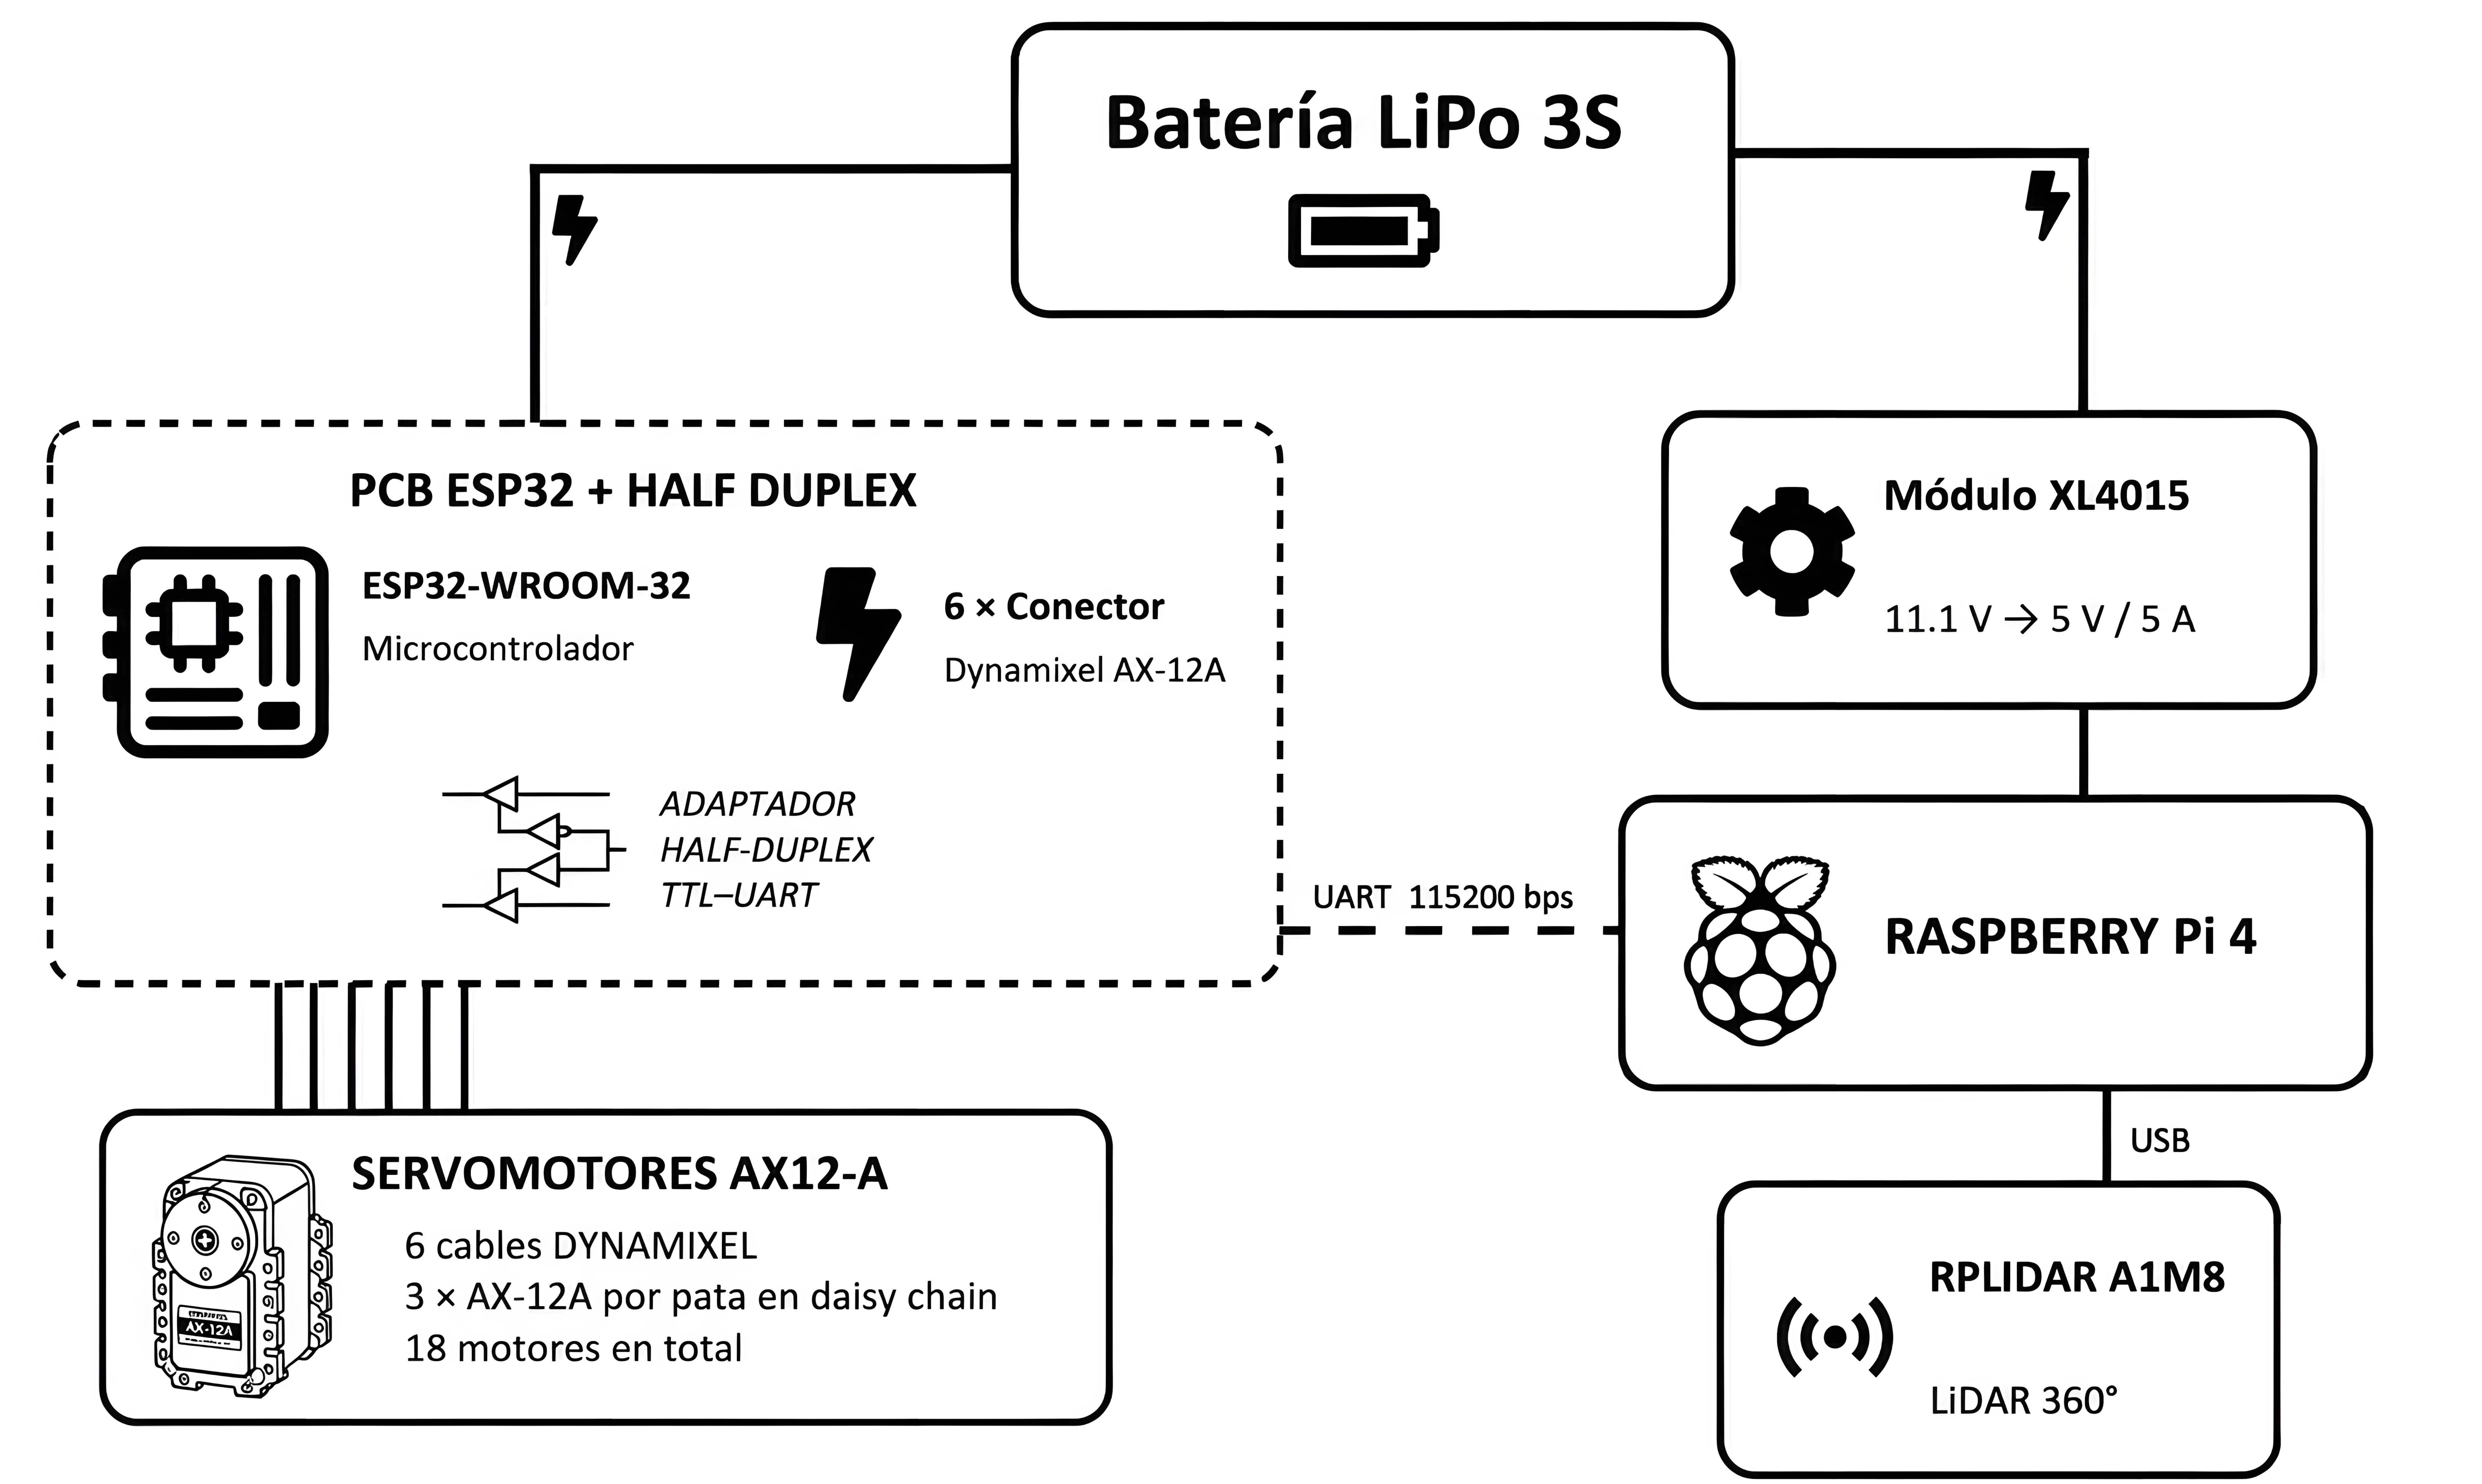
\includegraphics[width=\linewidth,height=1\textheight,keepaspectratio]{capitulos/cap3/figuras/DIAGRAMA ARQUITECTURA.jpg}
    \captionsetup{justification=centering}
    \caption{Arquitectura general de la plataforma hardware.}
    \footnotesize Fuente: Elaboración propia.
    \label{fig:arquitectura_hardware}
\end{figure}
\clearpage

La Figura~\ref{fig:arquitectura_hardware} presenta la arquitectura general de la
plataforma y las interconexiones entre sus subsistemas. Desde un punto de vista funcional, el sistema se organiza
en dos ramas claramente diferenciadas. La de alto nivel, que se ejecuta sobre la
Raspberry~Pi~4 \cite{raspberrypi4_datasheet}, donde residen los nodos ROS~2 y el
subsistema de percepción (Sección~\ref{sec:integracion_ros2}). Y la rama de bajo nivel, que se implementa sobre el
microcontrolador ESP32 \cite{esp32_datasheet} (Secciones~\ref{sec:hardware_bajo_nivel} y~\ref{subsec:organizacion_firmware}), responsable de la comunicación con
los actuadores y de la ejecución de las órdenes de movimiento hacia los servos DYNAMIXEL AX-12A \cite{ax12a_specs}. 

La alimentación global parte de una batería de polímero de litio (LiPo) de tres celdas (3S) y se distribuye
en dos ramas. La primera alimenta la PCB principal (Subsección~\ref{subsec:hw_half_duplex} y
\hyperref[anexo:documentacion_pcb]{Anexo~C}), que integra en un único soporte
físico la electrónica de control basada en el ESP32 y la distribución de potencia
hacia los 18 servomotores. Aunque ambas funciones conviven en la misma placa, el
diseño se ha planteado con una separación funcional entre la etapa de potencia
asociada a los motores y la lógica de control, con el fin de reducir interferencias
y facilitar la organización del sistema. Desde esta PCB se reparten alimentación y
datos mediante seis cables, uno por pata (Figura~\ref{fig:daisychain}).

La segunda rama incorpora un módulo comercial reductor de corriente continua (DC\nobreakdash-DC) basado en el
integrado XL4015 \cite{xl4015_datasheet}, que adapta la tensión nominal de la
batería ($11{,}1$~V) a $5$~V para alimentar la Raspberry~Pi~4. Este módulo se
seleccionó por su capacidad para suministrar hasta 5~A, suficiente para cubrir con
margen la demanda de corriente del subsistema de alto nivel. El sensor LiDAR
RPLIDAR~A1M8 \cite{rplidar_a1m8_datasheet}, conectado por USB a la
Raspberry~Pi~4, proporciona la medida del entorno con cobertura angular de 360°
(Subsección~\ref{subsec:lidar_ros2}).
La comunicación entre la Raspberry~Pi~4 y el ESP32 se realiza mediante un enlace
UART (\textit{Universal Asynchronous Receiver-Transmitter}) bidireccional a 115200~bps (Subsecciones~\ref{subsec:serial_bridge}
y~\ref{subsec:esp32_bridge_ros2}), lo que permite desacoplar la toma de decisiones
de alto nivel del control de bajo nivel de los actuadores. 

La Figura~\ref{fig:montaje_hardware} muestra el montaje del robot y la
disposición de la electrónica de control y alimentación sobre el chasis.

\begin{figure}[H]
    \centering
    \begin{subfigure}[t]{0.48\textwidth}
        \centering
        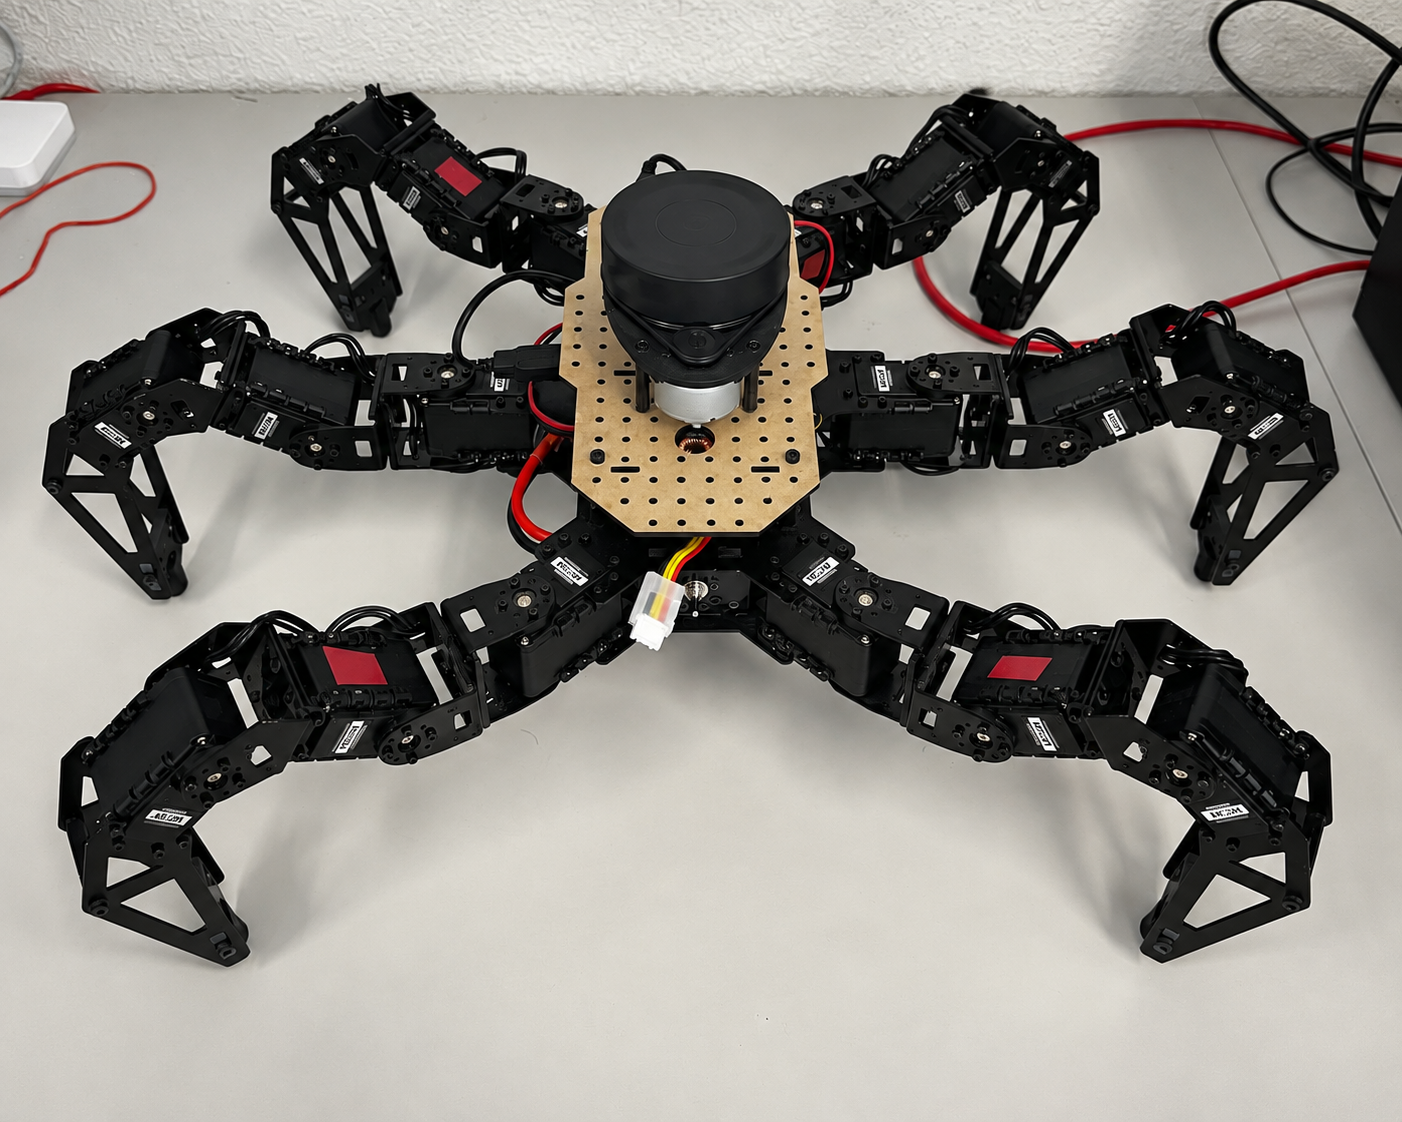
\includegraphics[width=\linewidth]
            {capitulos/cap3/figuras/montaje_hardware_general.png}
        \caption{Vista general del montaje hardware del robot.}
    \end{subfigure}
    \hfill
    \begin{subfigure}[t]{0.48\textwidth}
        \centering
        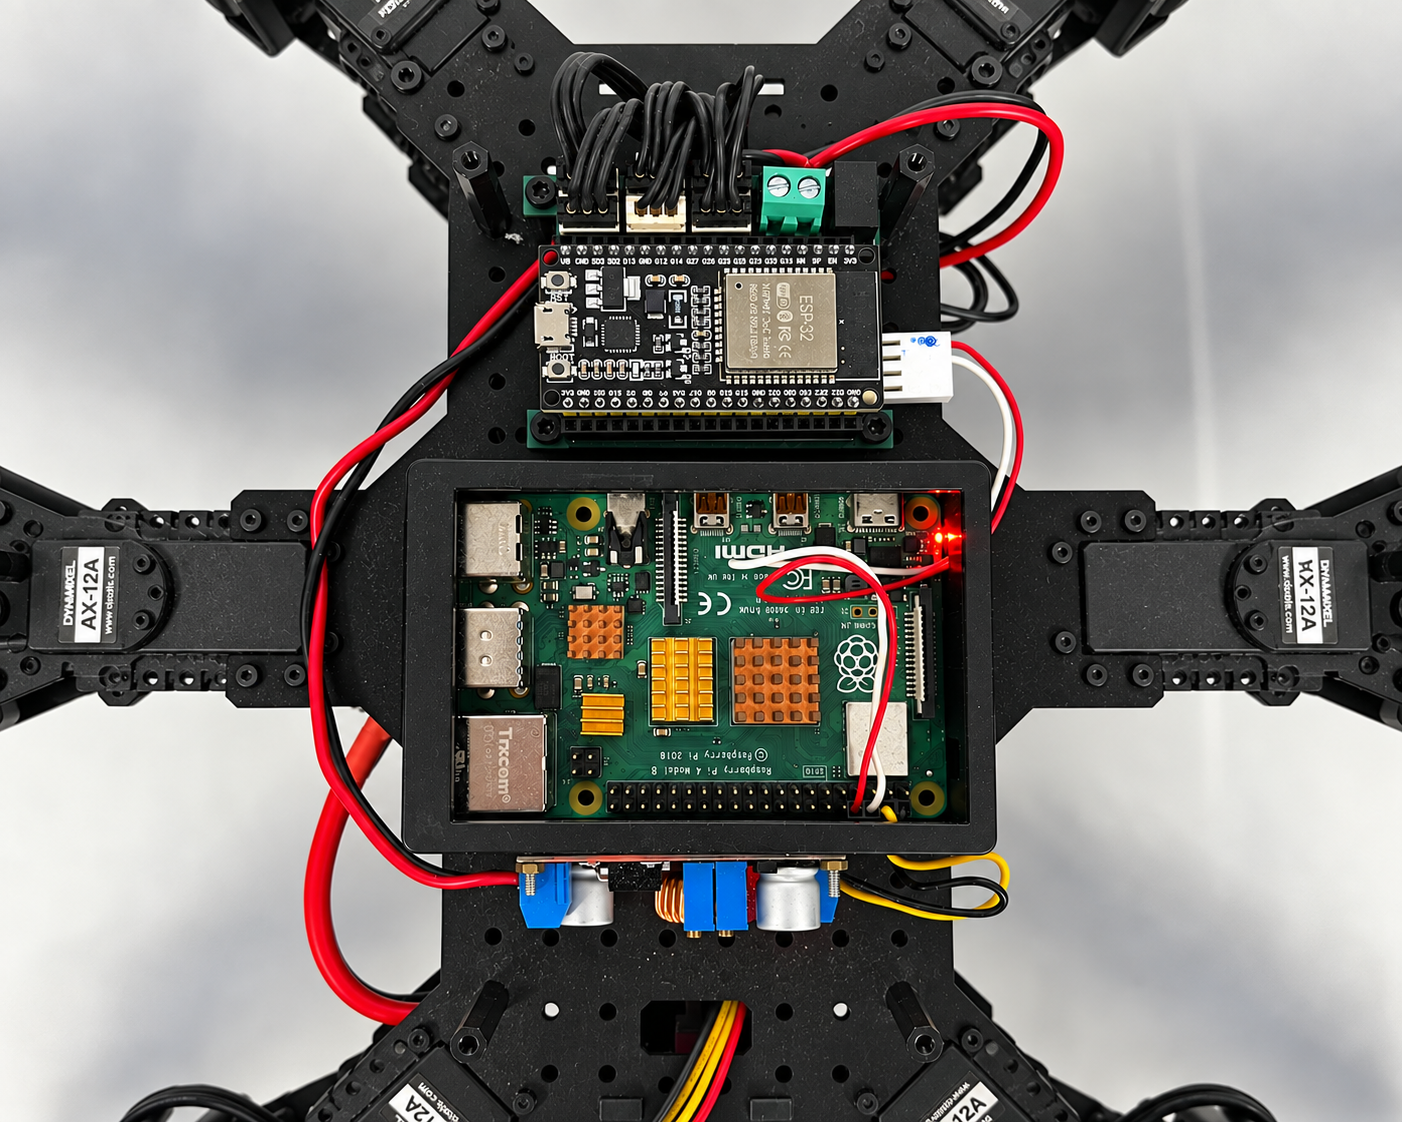
\includegraphics[width=\linewidth]
            {capitulos/cap3/figuras/montaje_hardware_detalle.png}
        \caption{Detalle de la electrónica de control y alimentación.}
    \end{subfigure}
    \captionsetup{justification=centering}
    \caption{Montaje hardware del hexápodo: vista general y detalle de la
    electrónica integrada.}
    {\centering\footnotesize Fuente: Elaboración propia.\par}
    \label{fig:montaje_hardware}
\end{figure}

\newpage
\section{Hardware de bajo nivel y control de actuadores}
\label{sec:hardware_bajo_nivel}

El subsistema de bajo nivel concentra los elementos responsables del control directo
del robot: los servomotores, el microcontrolador, la electrónica de adaptación y el
firmware ejecutado sobre el ESP32. Es conveniente presentarlo antes que el subsistema de alto nivel, ya que
constituye la base funcional sobre la que se apoya la capa ROS~2.

\subsection{Servomotores DYNAMIXEL AX-12A}
\label{subsec:servomotores_ax12a}

\begin{wrapfigure}[14]{r}{0.30\textwidth}
  \vspace{-0.3\baselineskip}
  \centering
  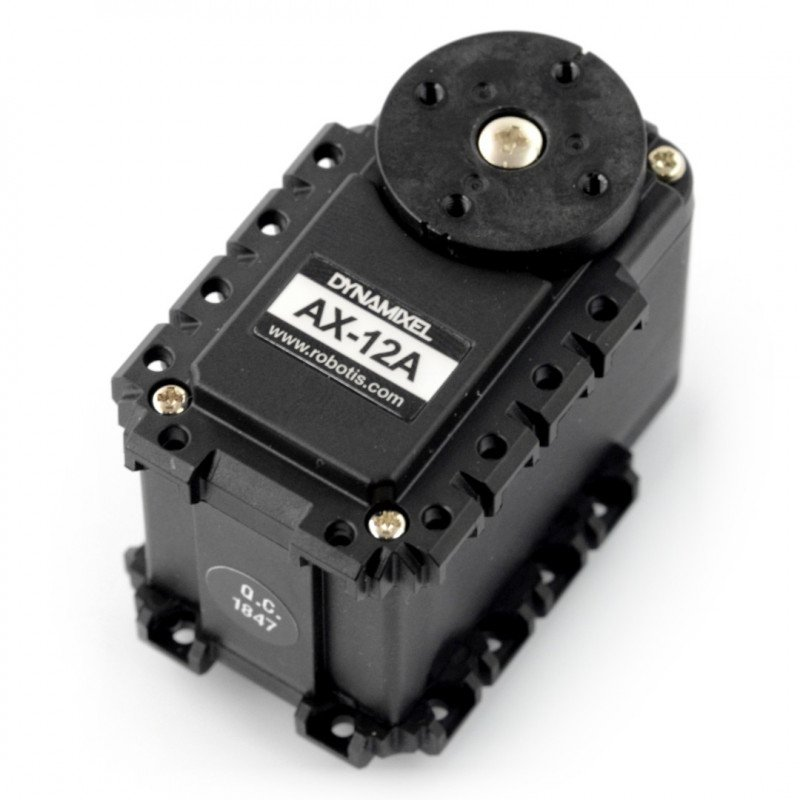
\includegraphics[width=0.90\linewidth,trim=0.7cm 0.7cm 0.7cm 0.7cm,clip]{capitulos/cap3/figuras/ax-12a.jpg}
  \captionsetup{justification=centering}
  \caption{Actuador DYNAMIXEL AX-12A.}
  \footnotesize Fuente: e-Manual de ROBOTIS~\cite{ax12a_specs}.
  \label{fig:ax12a}
\end{wrapfigure}

En este TFG se emplean servomotores DYNAMIXEL AX-12A \cite{ax12a_specs}
(Figura~\ref{fig:ax12a}),
que integran en un único módulo el motor DC con reductora, la electrónica de
potencia, el control interno y la sensórica necesaria para proporcionar
realimentación del estado del actuador. Desde el punto de vista mecánico, el actuador incorpora una reductora de
relación $254{:}1$ que le permite entregar un par de parada de $1{,}5$~N$\cdot$m
alimentado a $12$~V, con una velocidad máxima en vacío de $59$~rpm. Su sensor
interno discretiza el giro en 1024 niveles. Además, eléctricamente admite un rango de operación
de $9$ a $12$~V.

La conexión de cada actuador consiste en un cable de tres hilos que
agrupa la alimentación (VDD), la masa (GND) y la línea de datos, de manera que
potencia y comunicación comparten el mismo mazo de cable. 

\begin{figure}[hbtp]
    \centering
    \captionsetup{justification=centering}
    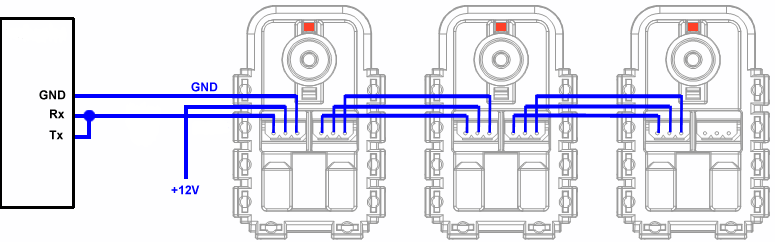
\includegraphics[width=0.8\linewidth]{capitulos/cap3/figuras/DaisyChain.png}
    \caption{Topología de conexión en cadena (\textit{daisy-chain}).}
    \footnotesize Fuente: Elaboración propia.
    \label{fig:daisychain}
\end{figure}

Tal y como muestra la Figura~\ref{fig:daisychain}, desde el concentrador de seis
puertos de la PCB los 18 actuadores se distribuyen en seis ramas, una por pata,
con tres servos conectados en topología \textit{daisy-chain} en cada una de
ellas. Dado que todos comparten físicamente la misma línea de datos, resulta
necesario asignar un identificador único a cada actuador. La
Tabla~\ref{tab:motor_ids} recoge esta asignación en función de la pata y de la
articulación correspondiente:

\begin{table}[H]
    \centering
    \footnotesize
    \captionsetup{justification=centering}
    \renewcommand{\arraystretch}{1.1}
    \rowcolors{2}{black!3}{white}
    \begin{tabular}{@{} l c c c @{\hspace{1.2cm}} l c c c @{}}
        \toprule
        Pata & Coxa & Fémur & Tibia &
        Pata & Coxa & Fémur & Tibia \\
        \midrule
        Izq. delantera (LT) & 1  & 3  & 5  & Der. delantera (RT) & 2  & 4  & 6  \\
        Izq. media (LM)     & 13 & 15 & 17 & Der. media (RM)     & 14 & 16 & 18 \\
        Izq. trasera (LB)   & 7  & 9  & 11 & Der. trasera (RB)   & 8  & 10 & 12 \\
        \bottomrule
    \end{tabular}
    \caption{Mapa de asignación de IDs de los actuadores.}
    \label{tab:motor_ids}
\end{table}

\subsection{Bus DYNAMIXEL y protocolo de comunicación}

La comunicación con los servomotores se realiza a través de un bus serie
propietario asíncrono \textit{half-duplex} sobre una única línea de datos.
Esta arquitectura permite compartir alimentación, masa y canal de
comunicaciones entre múltiples dispositivos, reduciendo de forma significativa
el cableado del robot. Sobre este medio físico se emplea el protocolo
DYNAMIXEL 1.0~\cite{ref_protocolo}, que define el formato de las tramas serie
intercambiadas entre el controlador y los actuadores. Aunque existe una versión
2.0, los AX-12A utilizados en este TFG solo son compatibles con la versión
1.0, de modo que su uso viene impuesto por el propio hardware. La comunicación
se articula en dos tipos de paquetes: el paquete de instrucción, enviado por el
controlador, y el paquete de estado, devuelto por el actuador como respuesta.

\paragraph{Paquete de instrucción}

El paquete de instrucción tiene la siguiente estructura:

\begin{equation}
\label{eq:dynamixel_instruction}
[\underbrace{\texttt{0xFF}\ \texttt{0xFF}}_{\text{Header}} |
\underbrace{\texttt{ID}}_{\text{ID}} |
\underbrace{\texttt{LEN}}_{\text{Longitud}} |
\underbrace{\texttt{INST}}_{\text{Instrucción}} |
\underbrace{\texttt{P}_1 \cdots \texttt{P}_N}_{\text{Parámetros}} |
\underbrace{\texttt{CSUM}}_{\text{Checksum}}]
\end{equation}

\begin{itemize}
    \item Header (\texttt{0xFF 0xFF}): dos bytes fijos que marcan el inicio
    de toda trama.
    \item ID: identificador del actuador destinatario (0--253). El valor
    especial \texttt{0xFE} es la dirección de \textit{broadcast}, que permite dirigirse
    a todos los actuadores simultáneamente.
    \item LEN: número de bytes restantes en el paquete, calculado como
    $N_{\text{parámetros}} + 2$.
    \item INST: código de la instrucción a ejecutar. La Tabla~\ref{tab:dynamixel_inst}
    recoge las principales.
    \item Parámetros: datos asociados a la instrucción.
    \item CSUM: suma de verificación del paquete, calculada como:
    \vspace{+0.2\baselineskip}
    \[
    \texttt{CSUM} = \overline{\texttt{ID} + \texttt{LEN} + \texttt{INST} + \texttt{P}_1 + \cdots + \texttt{P}_N}
    \]
\end{itemize}

\vspace{-0.5\baselineskip}
\begin{table}[H]
    \centering
    \footnotesize
    \captionsetup{justification=centering}
    \renewcommand{\arraystretch}{1.25}
    \rowcolors{2}{black!3}{white}
    \begin{tabularx}{\textwidth}{@{} >{\ttfamily}c c >{\raggedright\arraybackslash}X @{}}
        \toprule
        Código & Nombre & Descripción \\
        \midrule
        0x01 & Ping        & Comprueba la presencia de un actuador en el bus. \\
        0x02 & Read Data   & Lee uno o varios bytes consecutivos del mapa de memoria. \\
        0x03 & Write Data  & Escribe uno o varios bytes en el mapa de memoria. \\
        0x04 & Reg Write   & Registra una escritura pendiente, ejecutada al recibir Action. \\
        0x05 & Action      & Ejecuta la escritura registrada previamente con Reg Write. \\
        0x06 & Reset       & Restaura la configuración del actuador a sus valores de fábrica. \\
        0x83 & Sync Write  & Escribe simultáneamente en múltiples actuadores en una sola trama. \\
        \bottomrule
    \end{tabularx}
    \caption{Instrucciones principales del protocolo DYNAMIXEL 1.0.}
    \label{tab:dynamixel_inst}
\end{table}

\vspace{-0.5\baselineskip}

\textit{Sync Write} (\texttt{0x83}) resulta especialmente relevante en este
TFG. Su finalidad es escribir, en una única trama, un mismo bloque de
registros sobre múltiples actuadores. Para ello se emplea la dirección de
\textit{broadcast} (\texttt{0xFE}) y se indica la dirección inicial del
registro, la longitud del bloque que se desea escribir y, a continuación, una
secuencia formada por el identificador de cada servo y sus datos asociados.
Esto permite actualizar simultáneamente los 18 actuadores sin que estos generen
paquetes de estado en respuesta, al tratarse de una transmisión en
\textit{broadcast}.

\paragraph{Paquete de estado}

Tras recibir y procesar una instrucción, el actuador devuelve un paquete de estado con 
la siguiente estructura:

\begin{equation}
\label{eq:dynamixel_status}
[\underbrace{\texttt{0xFF}\ \texttt{0xFF}}_{\text{Header}} |
\underbrace{\texttt{ID}}_{\text{ID}} |
\underbrace{\texttt{LEN}}_{\text{Longitud}} |
\underbrace{\texttt{ERR}}_{\text{Error}} |
\underbrace{\texttt{P}_1 \cdots \texttt{P}_N}_{\text{Parámetros}} |
\underbrace{\texttt{CSUM}}_{\text{Checksum}}]
\end{equation}

El byte de error permite detectar condiciones anómalas en tiempo real sin necesidad de sensores externos. Cada bit corresponde a un tipo de error independiente (Figura~\ref{fig:ax12_errors}).

\begin{figure}[H]
    \centering
    \captionsetup{justification=centering}
    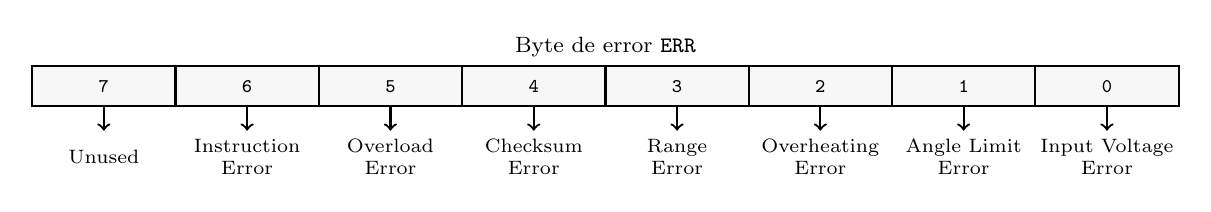
\begin{tikzpicture}[x=1.82cm,y=0.82cm,font=\scriptsize]
        \node[font=\footnotesize] at (4,0.92) {Byte de error \texttt{ERR}};

        \foreach \x/\b in {0/7,1/6,2/5,3/4,4/3,5/2,6/1,7/0} {
            \draw[thick, fill=black!3] (\x,0) rectangle ++(1,0.62);
            \node at (\x+0.5,0.31) {\texttt{\b}};
            \draw[->, thick] (\x+0.5,0) -- (\x+0.5,-0.38);
        }

        \node[align=center, text width=1.7cm] at (0.5,-0.78) {Unused};
        \node[align=center, text width=1.7cm] at (1.5,-0.78) {Instruction\\Error};
        \node[align=center, text width=1.7cm] at (2.5,-0.78) {Overload\\Error};
        \node[align=center, text width=1.7cm] at (3.5,-0.78) {Checksum\\Error};
        \node[align=center, text width=1.7cm] at (4.5,-0.78) {Range\\Error};
        \node[align=center, text width=1.7cm] at (5.5,-0.78) {Overheating\\Error};
        \node[align=center, text width=1.7cm] at (6.5,-0.78) {Angle Limit\\Error};
        \node[align=center, text width=1.7cm] at (7.5,-0.78) {Input Voltage\\Error};
    \end{tikzpicture}

    \caption{Distribución de bits del byte de error del DYNAMIXEL AX-12A.}
    \label{fig:ax12_errors}
\end{figure}

\vspace{-1.5\baselineskip}
\subsection{Mapa de memoria del AX-12A y registros utilizados}

El AX-12A dispone de una memoria interna organizada en dos áreas con propiedades
distintas. Por un lado, la EEPROM, de carácter no volátil, almacena la
configuración del servo, como su identificador, la velocidad de transmisión, los límites
angulares o la temperatura máxima permitida. Por otro lado, la RAM (\textit{Random Access Memory}), de carácter volátil, refleja el estado en
tiempo real e incluye la posición objetivo, la velocidad de movimiento, la
posición actual del eje, la dirección y magnitud estimadas de la carga o la
temperatura interna, entre otros registros. La carga indicada por el actuador se
infiere a partir de su salida interna y, por tanto, no constituye una medida
directa de par.

La Tabla~\ref{tab:ax12_memory} recoge los registros más relevantes de ambas áreas,
indicando su dirección, tamaño, rango y tipo de acceso.

\begin{table}[H]
    \centering
    \scriptsize
    \captionsetup{justification=centering}
    \renewcommand{\arraystretch}{1.15}
    \rowcolors{2}{black!3}{white}
    \begin{tabularx}{\textwidth}{@{} c c c >{\raggedright\arraybackslash}X c c @{}}
        \toprule
        Área & Dir. & Bytes & Registro & Rango & Acceso \\
        \midrule
        \rowcolor{black!8}\multicolumn{6}{@{}l}{\quad Memoria no volátil (EEPROM) — configuración estática} \\
        \multirow{7}{*}{EEPROM}
        & 0x03 & 1 & ID                  & 0 -- 253     & R/W \\
        & 0x04 & 1 & Baud Rate           & 0 -- 254     & R/W \\
        & 0x06 & 2 & CW Angle Limit      & 0 -- 1023    & R/W \\
        & 0x08 & 2 & CCW Angle Limit     & 0 -- 1023    & R/W \\
        & 0x0B & 1 & Temperature Limit   & 0 -- 100~°C  & R/W \\
        & 0x11 & 1 & Alarm LED           & 0 -- 127     & R/W \\
        & 0x12 & 1 & Shutdown            & 0 -- 127     & R/W \\
        \midrule
        \rowcolor{black!8}\multicolumn{6}{@{}l}{\quad Memoria volátil (RAM) — estado dinámico en tiempo real} \\
        \multirow{12}{*}{RAM}
        & 0x18 & 1 & Torque Enable         & 0 -- 1            & R/W \\
        & 0x1A & 1 & CW Compliance Margin  & 0 -- 255           & R/W \\
        & 0x1B & 1 & CCW Compliance Margin & 0 -- 255           & R/W \\
        & 0x1C & 1 & CW Compliance Slope   & 0 -- 254           & R/W \\
        & 0x1D & 1 & CCW Compliance Slope  & 0 -- 254           & R/W \\
        & 0x1E & 2 & Goal Position         & 0 -- 1023         & R/W \\
        & 0x20 & 2 & Moving Speed          & 0 -- 1023         & R/W \\
        & 0x24 & 2 & Present Position      & 0 -- 1023         & R   \\
        & 0x26 & 2 & Present Speed         & 0 -- 2047         & R   \\
        & 0x28 & 2 & Present Load          & 0 -- 2047         & R   \\
        & 0x2A & 1 & Present Voltage       & 50 -- 160          & R   \\
        & 0x2B & 1 & Present Temperature   & 0 -- 100           & R   \\
        \bottomrule
    \end{tabularx}
    \caption{Mapa de memoria del DYNAMIXEL AX-12A (registros principales).}
    \label{tab:ax12_memory}
\end{table}

\begin{wrapfigure}[14]{r}{0.25\textwidth}
  \vspace{-0.6\baselineskip}
  \centering
  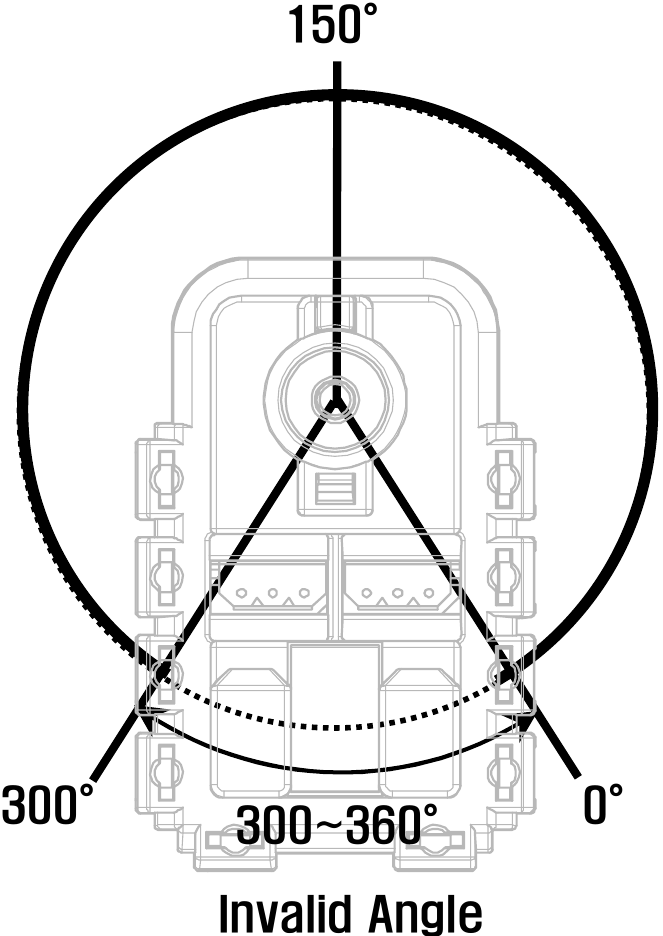
\includegraphics[width=0.9\linewidth]{capitulos/cap3/figuras/rango_angular.png}
  \captionsetup{justification=centering}
  \caption{Rango del AX-12A.}
  \footnotesize Fuente: e-Manual de ROBOTIS~\cite{ax12a_specs}.
  \label{fig:ax12_rango}
\end{wrapfigure}

Conviene detenerse primero en los registros de posición, ya que fijan las
unidades con las que trabaja el resto del mapa de memoria. Como muestra la
Figura~\ref{fig:ax12_rango}, en modo articulación el AX-12A dispone de un
recorrido útil de $300^\circ$, codificado mediante valores entre 0 y 1023. Esto
proporciona una resolución de $300^\circ/1023 \approx 0{,}293^\circ$ por unidad.
Los registros CW Angle Limit (0x06) y CCW Angle Limit (0x08) permiten
restringir dicho intervalo en el propio
actuador, de modo que las consignas situadas fuera de los límites configurados
no produzcan movimientos contra los topes mecánicos.

Resultan también especialmente relevantes los parámetros Compliance Margin y
Compliance Slope, ambos definidos con un registro independiente para cada
sentido de giro. La Figura~\ref{fig:ax12_compliance} ilustra el par de salida en
función del error de posición.

\begin{figure}[H]
    \centering
    \captionsetup{justification=centering}
    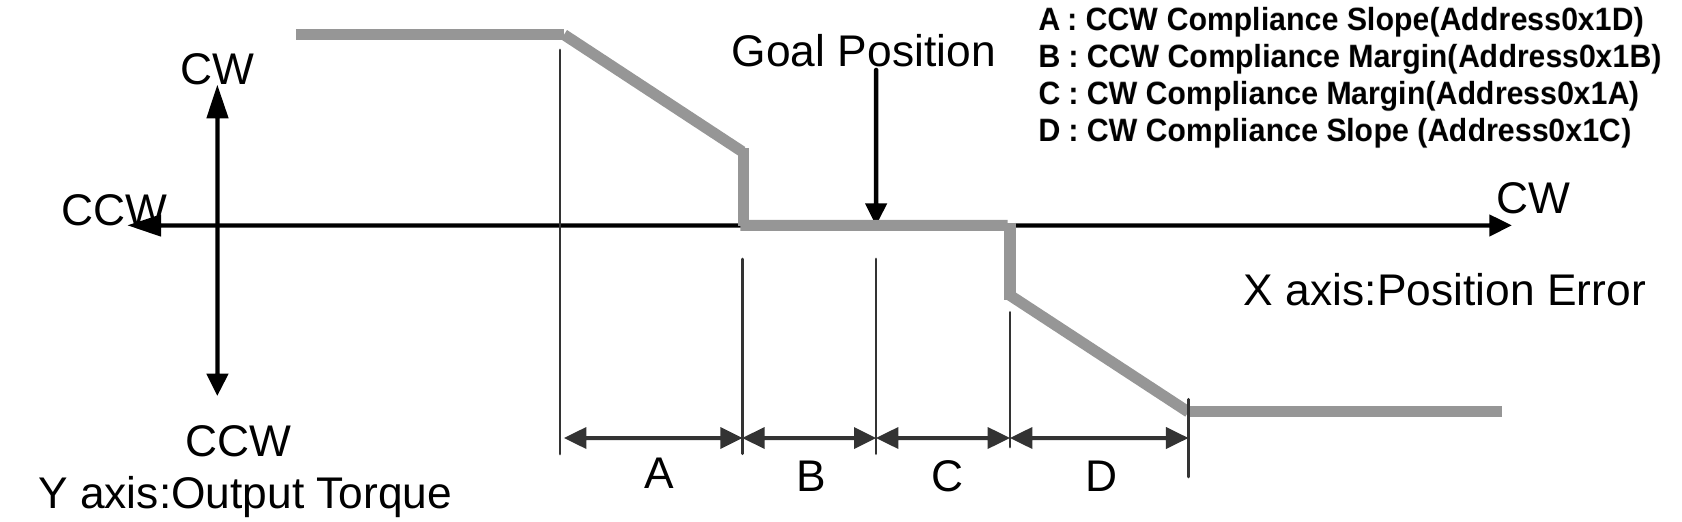
\includegraphics[width=0.75\linewidth]{capitulos/cap3/figuras/compliance.png}
    \caption{Perfil de par de salida en función del error de posición.}
    \footnotesize Fuente: e-Manual de ROBOTIS~\cite{ax12a_specs}.
    \label{fig:ax12_compliance}
\end{figure}

\vspace{-1.15\baselineskip}

El Compliance Margin define una zona muerta angular alrededor de la
posición objetivo, dentro de la cual el servo no genera par de corrección. El
Compliance Slope determina cómo crece dicho par una vez superada esa
zona y admite siete niveles discretos asociados a potencias de dos. Un margen
demasiado estrecho favorece las oscilaciones, el consumo y el calentamiento,
mientras que uno excesivo reduce la precisión del apoyo. De forma análoga, una
pendiente abrupta transmite los impactos a la estructura y una demasiado suave
reduce la capacidad de reacción frente al peso del robot. Atendiendo a este
equilibrio, se adoptaron empíricamente los valores 4 y 64. El primero equivale
aproximadamente a $1{,}17^\circ$ en cada sentido y produce una zona muerta total
de $2{,}35^\circ$. El segundo sitúa la pendiente en el penúltimo de los siete
escalones disponibles, proporcionando una respuesta más flexible cerca de la
consigna.

En la EEPROM también se configuran los registros Alarm LED y Shutdown con los
valores 0x25 y 0x04,
respectivamente. El indicador luminoso advierte así de errores de tensión,
temperatura y sobrecarga, mientras que la desconexión automática del par queda
reservada al sobrecalentamiento. De este modo, una incidencia transitoria de
alimentación o esfuerzo no provoca la pérdida simultánea de los apoyos del
robot.

Además, se ha desarrollado una herramienta de supervisión de los servomotores,
que se describirá posteriormente en la capa de alto nivel. Su base de bajo nivel
consiste en una única instrucción Read Data sobre el bloque de cuatro bytes
comprendido entre Present Load (0x28) y Present Temperature (0x2B): dos para la
carga estimada, uno para la tensión y otro para la temperatura. El paquete de
estado devuelto en esa misma transacción contiene además el byte de estado ERR.
Así se obtienen las variables de operación y las alarmas activas sin añadir otra
lectura al bus.

\subsection{Electrónica de adaptación al bus \textit{half-duplex}}
\label{subsec:hw_half_duplex}

La UART2 del ESP32~\cite{esp32_datasheet} dispone de líneas independientes de
transmisión y recepción y trabaja con niveles lógicos de $3{,}3$~V. En cambio,
los actuadores AX-12A comparten una única línea de datos TTL (\textit{Transistor-Transistor Logic}) de $5$~V y emplean
una comunicación \textit{half-duplex}~\cite{ax12a_specs}. La interfaz debe
resolver, por tanto, dos funciones: adaptar los niveles de tensión y conectar
alternativamente el transmisor o el receptor al bus de los servos. Esta
adaptación se integra en la PCB, que también
distribuye conjuntamente la alimentación y los datos, de forma similar a la
ArbotiX que se ha sustituido~\cite{arbotix_controller}.

Para entender el funcionamiento de la adaptación lógica y del \textit{buffer},
conviene comenzar por las tres señales que utiliza el microcontrolador:
\texttt{TX} (\texttt{GPIO16}), que transporta las instrucciones; \texttt{RX}
(\texttt{GPIO17}), que recibe los paquetes de estado; y \texttt{DIR}
(\texttt{GPIO2}), una salida digital que selecciona el sentido de la
comunicación. En el esquema de la Figura~\ref{fig:esquema_half_uart}, estas
redes se identifican como \texttt{TX3V3}, \texttt{RX3V3} y \texttt{DIR3V3}.

\vspace{-0.5\baselineskip}
\begin{figure}[H]
    \centering
    \captionsetup{justification=centering}
    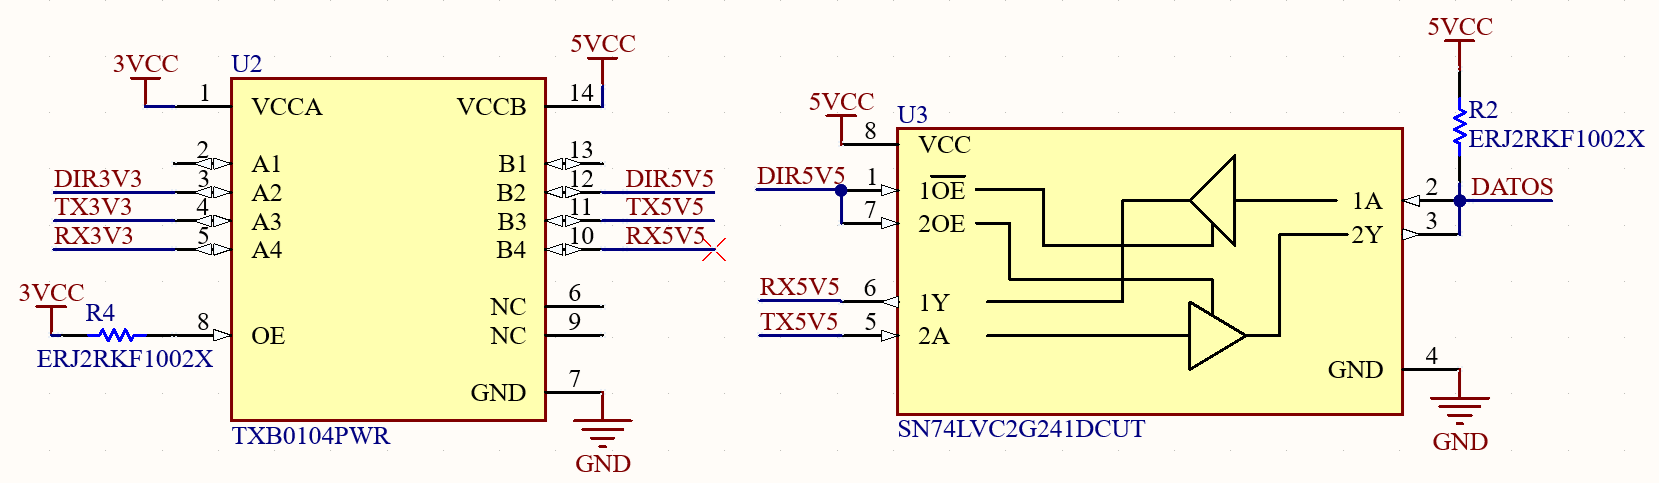
\includegraphics[width=0.9\linewidth]{capitulos/cap3/figuras/esquemahalfuart.png}
    \caption{Esquema de la interfaz de adaptación al bus \textit{half-duplex}.}
    \footnotesize Fuente: Elaboración propia mediante Altium Designer~\cite{altium_designer}.
    \label{fig:esquema_half_uart}
\end{figure}
\vspace{-1.2\baselineskip}

La primera etapa del circuito es un traductor bidireccional TXB0104PWR con
detección automática del sentido~\cite{txb0104_datasheet}. Su puerto A se
alimenta a $3{,}3$~V y el B a $5$~V. Tres de sus cuatro canales convierten las
señales anteriores en \texttt{DIR5V5}, \texttt{TX5V5} y \texttt{RX5V5}. La
resistencia R4 de $10$~k$\Omega$ mantiene activa la entrada \texttt{OE}, por lo
que el traductor permanece habilitado de forma permanente. 

Una vez adaptados los niveles, el buffer triestado SN74LVC2G241
convierte las líneas independientes de transmisión y recepción en una única
línea de datos~\cite{sn74lvc2g241_datasheet}. Como muestra la
Figura~\ref{fig:esquema_half_uart}, uno de sus canales conduce \texttt{TX5V5}
hacia \texttt{DATOS}, mientras que el otro conduce \texttt{DATOS} hacia
\texttt{RX5V5}. Ambos canales tienen habilitaciones de polaridad opuesta
gobernadas por \texttt{DIR5V5}. Con un nivel alto se habilita la transmisión y
el receptor queda en alta impedancia; con un nivel bajo se produce la situación
inversa. 

\begin{wraptable}[7]{r}{0.49\textwidth}
    \vspace{-0.8\baselineskip}
    \centering
    \captionsetup{justification=centering}
    \caption{Lógica de salidas del buffer.}
    \label{tab:direccion_halfduplex}
    \scriptsize
    \begin{tabular}{@{}ccc@{}}
        \toprule
        \shortstack{\texttt{DIR5V5}\\($\overline{\texttt{1OE}}=\texttt{2OE}$)}
            & \texttt{1Y} & \texttt{2Y} \\
        \midrule
        0 & \texttt{1A} (\texttt{DATOS}) & $Z$ \\
        1 & $Z$ & \texttt{2A} (\texttt{TX5V5}) \\
        \bottomrule
    \end{tabular}
    \vspace{-0.5\baselineskip}
\end{wraptable}

La Tabla~\ref{tab:direccion_halfduplex} resume esta selección, donde $Z$
representa el estado de alta impedancia de la salida deshabilitada. Además, la resistencia R2 
de $10$~k$\Omega$ actúa como \textit{pull-up} y mantiene \texttt{DATOS} a $5$~V cuando ningún dispositivo
conduce el bus. El estado de reposo programado es la recepción, con \texttt{DIR} a nivel bajo.
Para enviar una instrucción, el firmware eleva esta señal, escribe el paquete
en la UART y espera a que el último bit haya salido del periférico. Solo
entonces devuelve \texttt{DIR} a nivel bajo y habilita la recepción del paquete
de estado. Esta gestión del bus se implementa en el controlador de servomotores,
descrito en la Subsección~\ref{subsec:driver_ax12}.

\begin{wrapfigure}[14]{r}{0.35\textwidth}
    \vspace{-0.7\baselineskip}
    \centering
    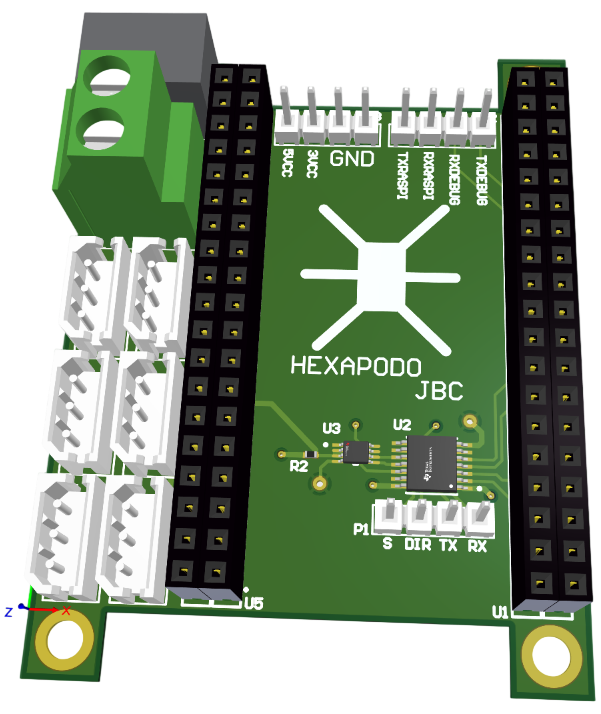
\includegraphics[width=0.94\linewidth]{capitulos/cap3/figuras/PCB1.png}
    \captionsetup{justification=centering}
    \caption{PCB en 3D.}
    \label{fig:pcb_3d_halfduplex}
    {\footnotesize Fuente: Altium Designer~\cite{altium_designer}.}
    \vspace{-0.4\baselineskip}
\end{wrapfigure}

La Figura~\ref{fig:pcb_3d_halfduplex} muestra la integración física del
circuito. El ESP32 se instala sobre dos tiras de zócalos para poder retirarlo sin
intervenir sobre los componentes soldados. El traductor de nivel y el
buffer triestado se sitúan entre ambas tiras, próximos a la cabecera
P1, que permite medir \texttt{DATOS}, \texttt{DIR}, \texttt{TX} y \texttt{RX}.
La línea de datos, la alimentación de los actuadores y la masa se conducen hasta
seis conectores Molex de tres vías, uno por pata.

La placa se ha diseñado con un apilado de cuatro capas: capa superior,
plano interno de masa, plano interno de alimentación y capa inferior. El plano
de masa proporciona una referencia común y un retorno de baja impedancia para
las señales. El plano de alimentación se divide en dos regiones aisladas:
\texttt{12VCC}, nombre asignado a la tensión no regulada de la batería LiPo 3S
($11{,}1$~V), y \texttt{5VCC}, generada por el
TSR~1-2450~\cite{tsr1_datasheet}. La primera
distribuye potencia a los actuadores y la segunda alimenta la lógica. Las capas
externas alojan los componentes, las señales y las conexiones locales con los
planos internos. La Figura~\ref{fig:pcb_capas_2d} muestra ambos trazados y su
superposición.

\vspace{-0.5\baselineskip}
\begin{figure}[H]
    \centering
    \begin{subfigure}[t]{0.27\textwidth}
        \centering
        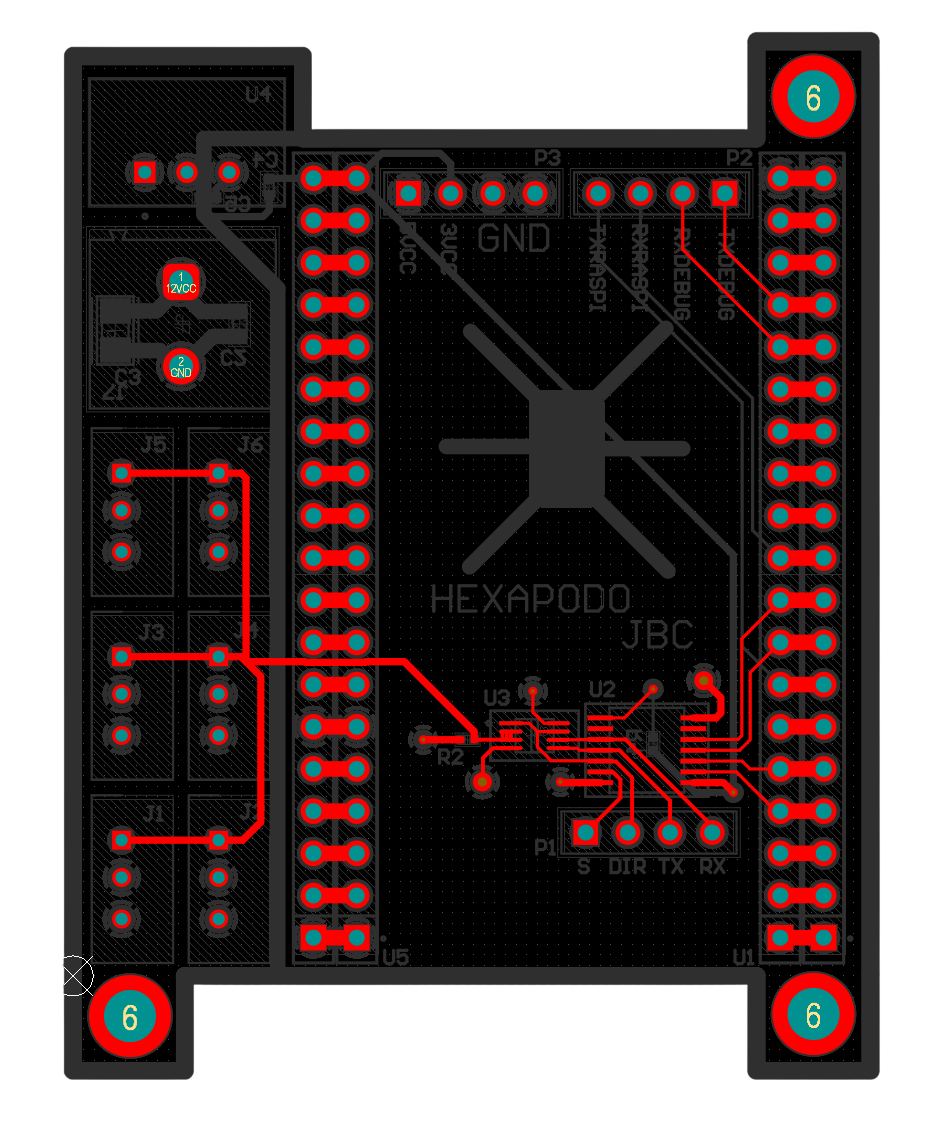
\includegraphics[width=\linewidth]{capitulos/cap3/figuras/toplayer.png}
        \caption{Trazado superior.}
        \label{fig:pcb_top_layer}
    \end{subfigure}
    \hfill
    \begin{subfigure}[t]{0.27\textwidth}
        \centering
        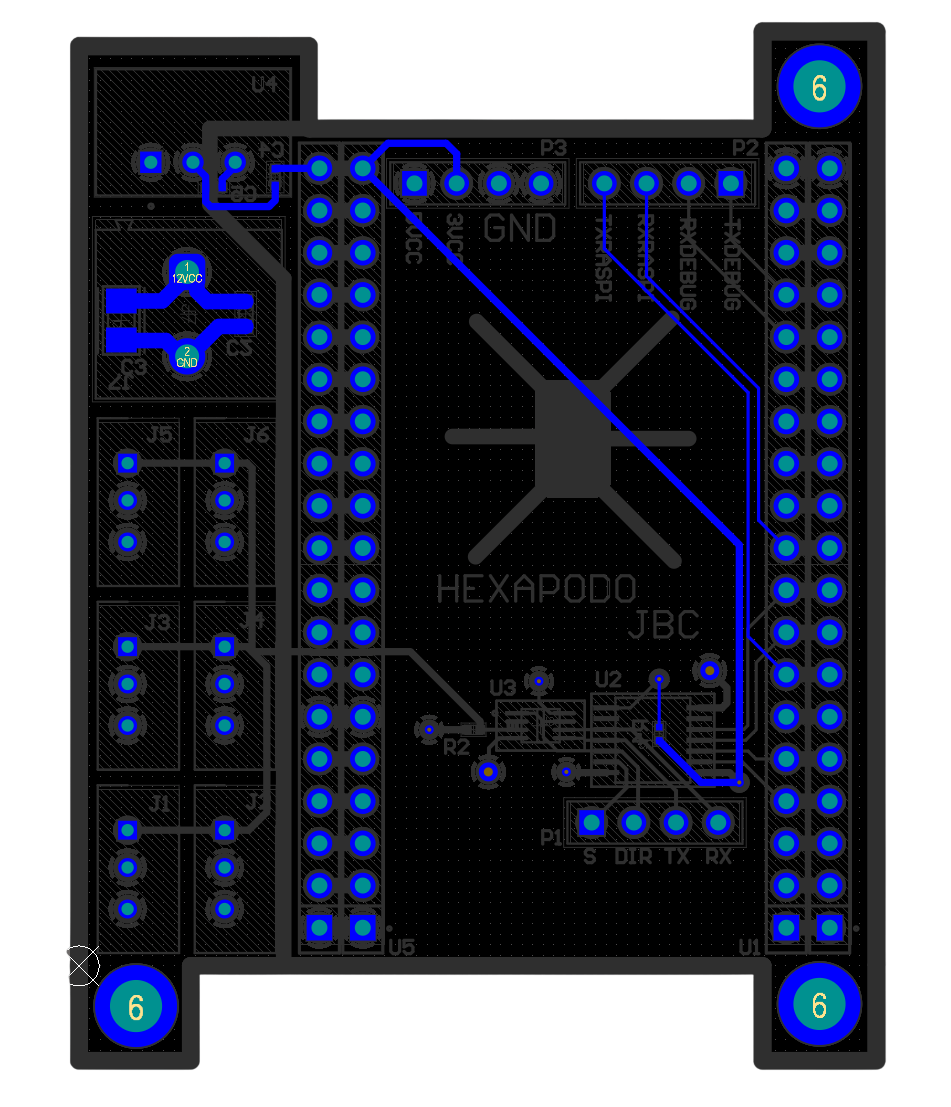
\includegraphics[width=\linewidth]{capitulos/cap3/figuras/bottonlayer.png}
        \caption{Trazado inferior.}
        \label{fig:pcb_bottom_layer}
    \end{subfigure}
    \hfill
    \begin{subfigure}[t]{0.27\textwidth}
        \centering
        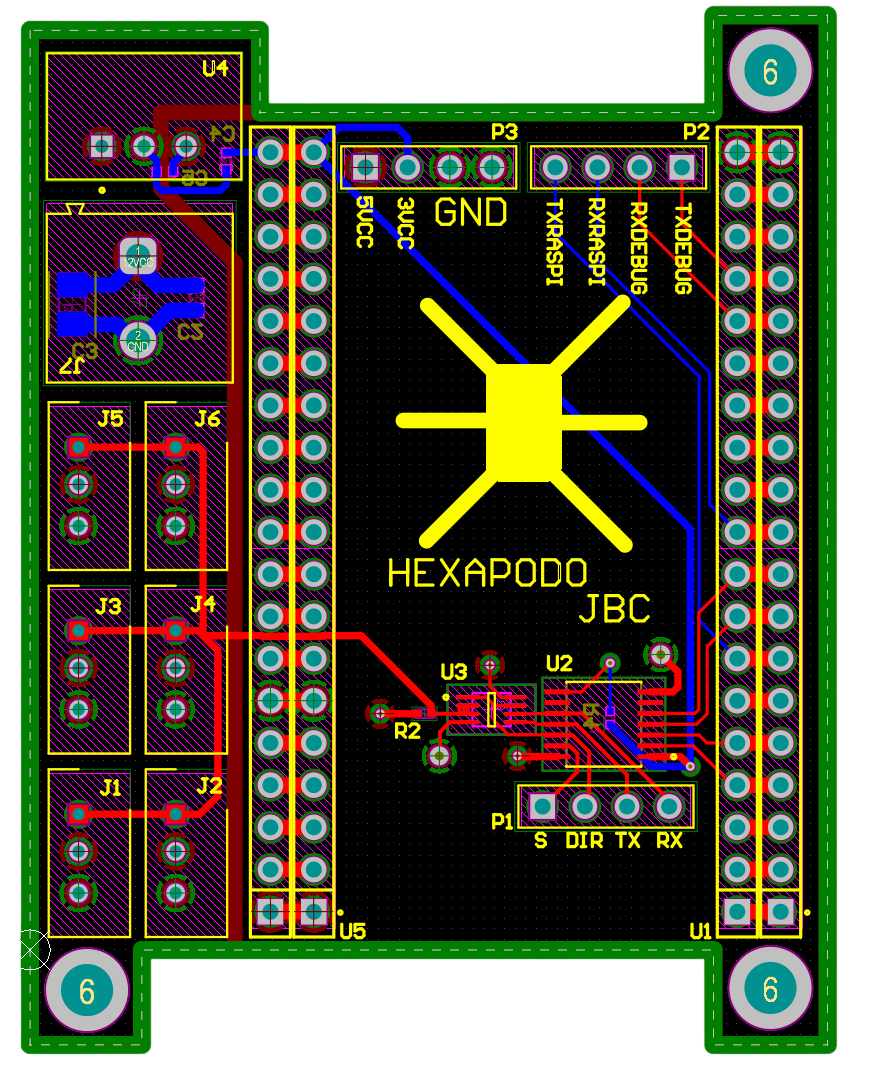
\includegraphics[width=\linewidth]{capitulos/cap3/figuras/pcb2d.png}
        \caption{Superposición 2D.}
        \label{fig:pcb_2d_combinada}
    \end{subfigure}
    \captionsetup{justification=centering}
    \caption{Encaminado en las capas externas de la PCB.}
    \label{fig:pcb_capas_2d}
    {\footnotesize Fuente: Altium Designer~\cite{altium_designer}.}
\end{figure}
\vspace{-1\baselineskip}

\begin{wrapfigure}[11]{r}{0.65\textwidth}
    \vspace{-0.7\baselineskip}
    \centering
    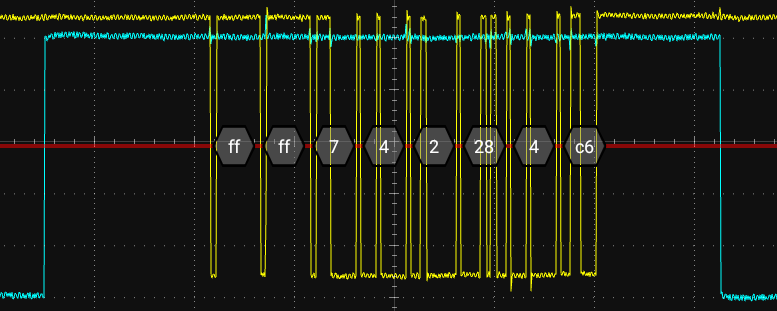
\includegraphics[width=0.98\linewidth]{capitulos/cap3/figuras/dirytx.png}
    \captionsetup{justification=centering}
    \caption{Captura de instrucción Read.}
    \label{fig:osciloscopio_dir_datos}
    {\footnotesize Fuente: Elaboración propia mediante osciloscopio RIGOL~\cite{rigol_dho800_datasheet}.}
\end{wrapfigure}


{\rightskip=0pt plus 2em
La Figura~\ref{fig:osciloscopio_dir_datos} muestra una captura de osciloscopio. La señal \texttt{DATOS} se representa en el canal~1 (amarillo) y la señal \texttt{DIR}, en el canal~2 (cian), con escalas de $20~\mu\text{s}/\text{div}$ y $1~\text{V}/\text{div}$, con un desplazamiento vertical para facilitar su identificación. Se observa cómo \texttt{DIR} pasa a nivel alto antes del inicio de la trama de lectura y permanece en dicho estado durante toda la transmisión. Tras el último bit, retorna a nivel bajo, conmutando el circuito al estado de escucha para recibir la respuesta del servomotor al que se dirige la instrucción.\par}


\newpage
\subsection{Módulo de acceso a los servomotores (\texttt{Firmware AX12A})}
\label{subsec:driver_ax12}

Una vez descritos los actuadores, el protocolo DYNAMIXEL y la electrónica de
adaptación \textit{half-duplex}, queda establecer la forma en que el firmware
del ESP32 accede al bus físico. Para ello se ha desarrollado el módulo
\texttt{ax12}, que reúne en una única interfaz las operaciones necesarias para
utilizar los 18 servomotores del hexápodo. El módulo constituye así la frontera
entre el hardware de actuación y los componentes software que se presentan en
los apartados posteriores.

La implementación se apoya en
\textit{Dynamixel2Espressif}~\cite{dynamixel2espressif}, un \textit{port} para
ESP-IDF publicado por hansj66 y derivado de la biblioteca
\textit{Dynamixel2Arduino}~\cite{dynamixel2arduino}, incorporado al proyecto
como copia local dentro del propio componente. Sobre esta base se define una
interfaz específica para la plataforma, de modo que el resto del firmware pueda
solicitar operaciones sobre los actuadores sin gestionar directamente la
construcción de paquetes DYNAMIXEL,  la configuración de la UART o la
conmutación de la línea de comunicación. La Figura~\ref{fig:arquitectura_ax12} resume su posición y responsabilidades:


\begin{figure}[H]
    \centering
    \makebox[\textwidth][c]{%
    \begin{tikzpicture}[
        font=\small,
        box/.style={
            draw=black,
            rounded corners=5pt,
            align=center,
            minimum height=0.95cm
        },
        own/.style={box, thick, fill=gray!10},
        external/.style={
            box,
            rounded corners=7pt,
            draw=black!62,
            line width=0.9pt,
            dash pattern=on 4pt off 2.6pt,
            fill=gray!4
        },
        layer/.style={text width=17.5cm},
        capability/.style={own, inner sep=5pt},
        tag/.style={
            draw=black,
            rounded corners=3pt,
            fill=white,
            inner sep=3pt
        },
        communication/.style={<->, thick, draw=black}
    ]

        \node[capability] (startup) at (-5.85,0) {%
            \begin{minipage}[t][2.95cm][t]{5.2cm}
                \centering
                \textbf{Puesta en marcha}\\[3pt]
                Inicialización, comprobación
                y configuración común\\[6pt]
                {\scriptsize\ttfamily ax12\_init}\\[-2pt]
                {\scriptsize\ttfamily ax12\_scan}\\[-2pt]
                {\scriptsize\ttfamily ax12\_configure\_eeprom\_ram}
            \end{minipage}%
        };

        \node[capability] (movement) at (0,0) {%
            \begin{minipage}[t][2.95cm][t]{5.2cm}
                \centering
                \textbf{Actuación}\\[3pt]
                Par individual y envío conjunto de
                posiciones\\[6pt]
                {\scriptsize\ttfamily ax12\_set\_torque}\\[-2pt]
                {\scriptsize\ttfamily ax12\_sync\_move\_deg\_speed}
            \end{minipage}%
        };

        \node[capability] (monitoring) at (5.85,0) {%
            \begin{minipage}[t][2.95cm][t]{5.2cm}
                \centering
                \textbf{Estado y mantenimiento}\\[3pt]
                Telemetría y lectura o escritura
                puntual de registros\\[6pt]
                {\scriptsize\ttfamily ax12\_read\_health}\\[-2pt]
                {\scriptsize\ttfamily ax12\_read\_register}\\[-2pt]
                {\scriptsize\ttfamily ax12\_write\_register}
            \end{minipage}%
        };

        \node[
            draw=black,
            very thick,
            rounded corners=6pt,
            fit=(startup)(movement)(monitoring),
            inner sep=7pt
        ] (ax12) {};

        % Rótulos montados sobre el borde superior del módulo.
        \node[tag, font=\small, anchor=west] (module-title)
            at ([xshift=0.8cm]ax12.north west) {\textbf{Módulo \texttt{ax12}}};

        \node[tag, font=\scriptsize\ttfamily, anchor=east] (files)
            at ([xshift=-0.8cm]ax12.north east) {ax12.h\quad ax12.cpp};

        \node[external, layer, below=0.70cm of ax12, minimum height=1.15cm]
            (bus) {
            \textbf{Biblioteca \textit{Dynamixel2Espressif} y enlace
            \textit{half-duplex}}\\
            Paquetes DYNAMIXEL~1.0 sobre el bus compartido con los 18
            servomotores AX-12A
        };

        \draw[communication] (ax12) --
            node[right,font=\footnotesize]{operaciones DYNAMIXEL} (bus);

    \end{tikzpicture}}
    \captionsetup{justification=centering}
    \caption[Posición y responsabilidades del módulo \texttt{ax12}]
    {Posición y responsabilidades del módulo \texttt{ax12} en el acceso a los
    actuadores.}
    \label{fig:arquitectura_ax12}
    {\footnotesize El código fuente y la documentación detallada de la API (\textit{Application Programming Interface}),
    generada mediante Doxygen~\cite{doxygen}, se encuentran disponibles en el
    repositorio del proyecto~\cite{repositorio_hexapodo}.}
\end{figure}

El módulo concentra en una única interfaz todo el ciclo de uso de los
actuadores, de modo que ningún otro componente del firmware necesita acceder
directamente al bus. Para el movimiento coordinado agrupa en una sola trama,
mediante la instrucción \textit{Sync Write}
(Tabla~\ref{tab:dynamixel_inst}), las consignas de los actuadores seleccionados
junto con una velocidad común, evitando una transacción independiente por
servomotor sobre un enlace que todos comparten. Además, las posiciones
expresadas en grados se convierten a los valores entre 0 y 1023 con que el
AX-12A codifica su recorrido (Tabla~\ref{tab:ax12_memory}).

Por último, cabe destacar que el conocimiento específico del AX-12A queda confinado aquí, en el único punto del firmware que incluye la biblioteca DYNAMIXEL y que manipula valores de registro. Sustituir los actuadores por un modelo distinto obligaría, por tanto, a reescribir la implementación de \texttt{ax12}, pero no la interfaz que utiliza el resto del
firmware, que seguiría solicitando posiciones en grados.

\newpage
\section{Implementación del firmware cinemático}
\label{subsec:organizacion_firmware}

Una vez se ha descrito el acceso al bus mediante el módulo
\hyperref[subsec:driver_ax12]{\texttt{ax12}} y su funcionamiento lógico y eléctrico, esta sección presenta el firmware que transforma las consignas de ROS~2 en referencias para los 18 servomotores. La implementación combina módulos cinemáticos, un estado compartido sincronizado
y tres tareas de FreeRTOS~\cite{freertos}. La
Figura~\ref{fig:organizacion_firmware} recorre este flujo hasta los
\mbox{AX-12A}.

\begin{figure}[H]
    \centering
    \makebox[\textwidth][c]{%
    \begin{tikzpicture}[
        >=stealth,
        font=\scriptsize,
        every node/.style={align=center},
        box/.style={
            rectangle,
            draw=black,
            rounded corners=5pt,
            align=center,
            inner sep=5pt,
            minimum height=0.85cm
        },
        own/.style={box, thick, fill=gray!10},
        wide/.style={own, text width=6.4cm},
        task/.style={own, text width=4.6cm, minimum height=1.15cm},
        module/.style={own, font=\scriptsize, text width=2.85cm, minimum height=1.05cm},
        base/.style={own, font=\scriptsize, text width=4.10cm, minimum height=1.05cm},
        external/.style={
            box,
            rounded corners=7pt,
            draw=black!62,
            line width=0.9pt,
            dash pattern=on 4pt off 2.6pt,
            fill=gray!4
        },
        tag/.style={
            draw=black,
            rounded corners=3pt,
            fill=white,
            inner sep=3pt
        },
        flow/.style={->, thick, draw=black},
        shared/.style={<->, thick, draw=black},
        dependency/.style={->, thick, dashed, draw=black!65}
    ]

        \node[external, text width=2.1cm] (raspi) at (0,0.35) {
            \textbf{ROS~2}
        };

        \node[wide] (serial) at (0,-1.50) {
            \textbf{\texttt{serial\_bridge}}\\
            protocolo de comandos de texto sobre UART1\\[-1pt]
            {\tiny Subsección~\ref{subsec:serial_bridge}}
        };

        \node[wide] (controller) at (0,-3.30) {
            \textbf{\texttt{robot\_controller}}\\
            API de estado compartido y sincronización de tareas\\[-1pt]
            {\tiny Subsección~\ref{subsec:robot_controller}}
        };

        \node[task] (locomotion) at (0,-5.45) {
            \textbf{\texttt{locomotion\_task}}\\
            tarea que ejecuta un bucle periódico de 20~ms para la marcha y la cinemática\\[-1pt]
            {\tiny Subsección~\ref{subsec:locomotion_task}}
        };

        \node[own, text width=4.00cm, minimum height=1.15cm]
            (diagnostic) at (5.25,-5.45) {
            \textbf{\texttt{diagnostic}}\\
            Supervisión de los servomotores\\[-1pt]
            {\tiny Subsección~\ref{subsec:diagnostic}}
        };

        \node[own, font=\scriptsize, text width=3.20cm,
            minimum height=0.95cm] (matrix) at (-6.00,-4.30) {
            \textbf{\texttt{matrix\_math}}\\
            álgebra espacial\\[-1pt]
            {\tiny Subsección~\ref{subsec:matrix_math}}
        };

        \node[own, font=\scriptsize, text width=3.20cm,
            minimum height=0.95cm] (config) at (-6.00,-5.60) {
            \textbf{\texttt{leg\_config}}\\
            geometría y calibración\\[-1pt]
            {\tiny Subsección~\ref{subsec:leg_config}}
        };

        \node[
            draw=black!62,
            rounded corners=5pt,
            dash pattern=on 4pt off 2.6pt,
            fit=(matrix)(config),
            inner xsep=7pt,
            inner ysep=9pt
        ] (auxiliaries) {};

        \node[tag, font=\scriptsize, anchor=west]
            at ([xshift=0.2cm]auxiliaries.north west)
            {\textbf{Módulos auxiliares}};

        \node[module] (posture) at (-6.15,-8.25) {
            \textbf{\texttt{posture\_engine}}\\
            suavizado de postura\\[-1pt]
            {\tiny Subsección~\ref{subsec:posture_engine}}
        };

        \node[module] (body) at (-2.05,-8.25) {
            \textbf{\texttt{body\_kinematics}}\\
            postura y odometría\\[-1pt]
            {\tiny Subsección~\ref{subsec:body_kinematics}}
        };

        \node[module] (gait) at (2.05,-8.25) {
            \textbf{\texttt{gait\_engine}}\\
            fases y trayectorias\\[-1pt]
            {\tiny Subsección~\ref{subsec:gait_engine}}
        };

        \node[module] (leg) at (6.15,-8.25) {
            \textbf{\texttt{leg\_kinematics}}\\
            IK de las seis patas\\[-1pt]
            {\tiny Subsección~\ref{subsec:leg_kinematics}}
        };

        \node[
            draw=black,
            rounded corners=5pt,
            fit=(posture)(body)(gait)(leg),
            inner xsep=7pt,
            inner ysep=9pt
        ] (kinematics) {};

        \node[tag, font=\scriptsize, anchor=west]
            at ([xshift=0.45cm]kinematics.north west)
            {\textbf{Cálculo cinemático}};

        \node[
            draw=black,
            very thick,
            rounded corners=6pt,
            fit=(serial)(controller)(locomotion)(diagnostic)(auxiliaries)(kinematics),
            inner xsep=9pt,
            inner ysep=11pt
        ] (firmware) {};

        \node[tag, font=\small, anchor=west]
            at ([xshift=0.4cm]firmware.north west)
            {\textbf{Firmware cinemático}};

        % Nodo hardware desplazado abajo de cinemática y fuera del firmware
        \node[external, font=\small, text width=2.60cm]
            (hardware) at (0,-10.50) {
            \textbf{AX-12A}\\[-1pt]
            {\tiny Subsección~\ref{subsec:servomotores_ax12a}}
        };

        \draw[shared] (raspi) -- (serial);
        \draw[shared] (serial) -- (controller);
        \draw[shared] (controller) -- (locomotion);
        \draw[shared] (controller) -- (diagnostic);
        \draw[flow] (locomotion) -- (diagnostic);

        \draw[flow] (locomotion.south) -- (kinematics.north);

        % Flecha redibujada para bajar verticalmente al nodo de hardware
        \draw[flow] (kinematics.south) -- (hardware.north);

        \draw[flow] (posture) -- (body);
        \draw[shared] (body) -- (gait);
        \draw[flow] (gait) -- (leg);

    \end{tikzpicture}}
    \captionsetup{justification=centering}
    \caption[Organización del firmware del hexápodo]
    {Módulos y flujos principales del firmware del hexápodo. Las flechas simples
    representan el flujo de datos; las dobles, un intercambio bidireccional.}
    \label{fig:organizacion_firmware}
\end{figure}
\vspace{-1\baselineskip}

Las órdenes recibidas por
\hyperref[subsec:serial_bridge]{\texttt{serial\_bridge}} se trasladan a
\hyperref[subsec:robot_controller]{\texttt{robot\_controller}}, que conserva el
estado compartido y sincroniza su acceso. En sentido inverso, el puente devuelve
a ROS~2 la odometría y la telemetría. Cada 20~ms,
\hyperref[subsec:locomotion_task]{\texttt{locomotion\_task}} obtiene los
objetivos vigentes y ejecuta sucesivamente
\hyperref[subsec:posture_engine]{\texttt{posture\_engine}},
\hyperref[subsec:body_kinematics]{\texttt{body\_kinematics}},
\hyperref[subsec:gait_engine]{\texttt{gait\_engine}} y
\hyperref[subsec:leg_kinematics]{\texttt{leg\_kinematics}}. El cálculo se realiza
sobre una copia provisional del estado. Si las seis soluciones resultan válidas,
el ciclo se confirma y las 18 referencias articulares se envían mediante una
única instrucción \textit{Sync Write}; de lo contrario, se conserva el último
estado válido. Los módulos
\hyperref[subsec:matrix_math]{\texttt{matrix\_math}} y
\hyperref[subsec:leg_config]{\texttt{leg\_config}} actúan como auxiliares y
aportan, respectivamente, las operaciones de álgebra espacial y los parámetros
de geometría.

Tras cada ciclo, \hyperref[subsec:locomotion_task]{\texttt{locomotion\_task}}
activa \hyperref[subsec:diagnostic]{\texttt{diagnostic}} para consultar la
telemetría o acceder a los registros de los actuadores, tareas necesarias por los esfuerzos electromecánicos a los que están sometidos los motores. Su menor prioridad reduce
la interferencia con el control periódico. La comunicación serie se ejecuta en el
núcleo~0 del ESP32, mientras que la locomoción y el diagnóstico se ejecutan en el
núcleo~1.


\subsection{Biblioteca de transformaciones espaciales (\texttt{matrix\_math})}
\label{subsec:matrix_math}

El módulo \texttt{matrix\_math} centraliza el álgebra tridimensional empleada
por la cinemática del cuerpo y de las patas y por el generador de marcha. Así,
todos ellos comparten representaciones y convenciones, se evita duplicar
operaciones y se facilitan implementaciones eficientes. La interfaz sigue la
Sección~\ref{sec:descripcion_espacial} y se resume en la
Figura~\ref{fig:arquitectura_matrix_math}.

\begin{figure}[H]
    \centering
    \makebox[\textwidth][c]{%
    \begin{tikzpicture}[
        font=\scriptsize,
        every node/.style={align=center},
        box/.style={
            rectangle,
            draw=black,
            rounded corners=5pt,
            align=center,
            inner sep=3pt
        },
        own/.style={box, thick, fill=gray!10},
        api/.style={
            own,
            font=\tiny,
            minimum height=2.50cm
        },
        vectorapi/.style={api, text width=2.45cm},
        matrixapi/.style={api, text width=4.95cm},
        rotationapi/.style={api, text width=3.80cm},
        transformapi/.style={api, text width=4.90cm},
        tag/.style={
            draw=black,
            rounded corners=3pt,
            fill=white,
            inner sep=3pt
        }
    ]

        \node[vectorapi] (vectors) at (-7.32,0) {
            {\scriptsize\textbf{Escalar/ Vector}}\\
            {\scriptsize\texttt{vec3}}\\[2pt]
            \texttt{scalar\_clamp}\\[-1pt]
            \texttt{scalar\_square}\\[-1pt]
            \texttt{vector3\_add}\\[-1pt]
            \texttt{vector3\_sub}
        };
        \node[matrixapi] (matrices) at (-3.29,0) {
            {\scriptsize\textbf{Matrices}}\\
            {\scriptsize\texttt{mat3}}\\[2pt]
            \texttt{matrix3\_identity}\\[-1pt]
            \texttt{matrix3\_multiply}\\[-1pt]
            \texttt{matrix3\_apply\_to\_vector}\\[-1pt]
            \texttt{matrix3\_transpose}\\[-1pt]
            \texttt{matrix3\_apply\_transpose\_to\_vector}~Ec.~\ref{eq:R_inv_RT}
        };
        \node[rotationapi] (rotations) at (1.42,0) {
            {\scriptsize\textbf{Rotaciones}}\\[2pt]
            \texttt{rotation\_matrix\_x}~Ec.~\ref{eq:Rzyx_producto_elementales}\\[-1pt]
            \texttt{rotation\_matrix\_y}~Ec.~\ref{eq:Rzyx_producto_elementales}\\[-1pt]
            \texttt{rotation\_matrix\_z}~Ec.~\ref{eq:Rzyx_producto_elementales}\\[-1pt]
            \texttt{rotation\_matrix\_from\_rpy}~Ec.~\ref{eq:Rypr_comp}
        };
        \node[transformapi] (transforms) at (6.10,0) {
            {\scriptsize\textbf{Transformaciones}}\\
            {\scriptsize\texttt{se3}}\\[2pt]
            \texttt{rigid\_transform\_identity}\\[-1pt]
            \texttt{rigid\_transform\_inverse}~Ec.~\ref{eq:T_inversa}\\[-1pt]
            \texttt{rigid\_transform\_from\_rpy\_xyz}~Ec.~\ref{eq:T_homogenea}\\[-1pt]
            \texttt{rigid\_transform\_compose}~Ec.~\ref{eq:concatenacion_T}\\[-1pt]
            \texttt{rigid\_transform\_apply\_to\_point}~Ec.~\ref{eq:transformacion_fundamental}
        };

        \node[
            draw=black,
            very thick,
            rounded corners=6pt,
            fit=(vectors)(matrices)(rotations)(transforms),
            inner xsep=6pt,
            inner ysep=5pt
        ] (module) {};

        \node[tag, font=\scriptsize, anchor=west]
            at ([xshift=0.35cm]module.north west)
            {\textbf{Módulo \texttt{matrix\_math}}};

        \node[tag, font=\tiny\ttfamily, anchor=east]
            at ([xshift=-0.35cm]module.north east)
            {matrix\_math.h};

    \end{tikzpicture}}
    \captionsetup{justification=centering,singlelinecheck=false}
    \caption[Organización de la biblioteca \texttt{matrix\_math}]
    {Tipos y familias de operaciones de la biblioteca \texttt{matrix\_math}.}
    \label{fig:arquitectura_matrix_math}
\end{figure}
\vspace{-1\baselineskip}

Aunque no se describen aquí todas las funciones de la biblioteca, su
funcionamiento, sus parámetros y sus valores de retorno se detallan junto al
código mediante Doxygen~\cite{doxygen}. Cabe destacar que, para matrices de
rotación, \texttt{matrix3\_transpose} obtiene la inversa
mediante la propiedad $R^{-1}=R^{T}$ de la
Ec.~\ref{eq:R_inv_RT}. La función
\texttt{matrix3\_apply\_transpose\_to\_vector} la aplica directamente a un
vector. La función
\texttt{rotation\_matrix\_from\_rpy} compone las rotaciones elementales según
la Ec.~\ref{eq:Rypr_comp}. Las transformaciones rígidas se almacenan con
el tipo \texttt{se3}, formado por una matriz de rotación $R$ y un
vector de traslación $t$. Así se evita almacenar la última fila constante
de la matriz homogénea de la Ec.~\ref{eq:T_homogenea}.

\subsection{Configuración de las patas (\texttt{leg\_config})}
\label{subsec:leg_config}

El módulo \texttt{leg\_config} reúne los parámetros que diferencian las seis
patas: los identificadores de los actuadores, la geometría y el anclaje al
chasis, los ajustes de montaje y los límites software. La configuración se
almacena en el array constante \texttt{g\_leg\_cfgs}, formado por seis
estructuras \texttt{leg\_cfg\_t}. Cada entrada contiene a su vez una estructura
\texttt{leg\_params} con las magnitudes geométricas. La
Figura~\ref{fig:arquitectura_leg_config} resume esta organización.

\begin{figure}[H]
    \centering
    \makebox[\textwidth][c]{%
    \begin{tikzpicture}[
        >=stealth,
        font=\scriptsize,
        every node/.style={align=center},
        field/.style={
            rectangle,
            draw=black,
            thick,
            rounded corners=4pt,
            fill=gray!7,
            font=\tiny,
            inner xsep=3pt,
            inner ysep=3pt,
            minimum height=2.00cm
        },
        array/.style={
            rectangle,
            draw=black,
            thick,
            rounded corners=4pt,
            fill=gray!18,
            text width=16.40cm,
            minimum height=1.05cm,
            inner xsep=3pt,
            inner ysep=2pt
        },
        identity/.style={field, text width=3.60cm},
        geometry/.style={field, text width=4.60cm},
        calibration/.style={field, text width=7.70cm},
        tag/.style={
            draw=black,
            rounded corners=3pt,
            fill=white,
            inner sep=3pt
        },
        flow/.style={->, thick, draw=black}
    ]

        \node[array] (array) at (0,0) {
            \textbf{Array constante de configuración} \quad
            \texttt{g\_leg\_cfgs[LEG\_COUNT]} : \texttt{leg\_cfg\_t[6]}\\[-1pt]
            \texttt{LT} · \texttt{LM} · \texttt{LB} ·
            \texttt{RB} · \texttt{RM} · \texttt{RT}
            \quad Tabla~\ref{tab:parametros_pata}\\[-1pt]
            {\tiny Índice \texttt{leg\_id\_t}: una entrada constante por pata}
        };

        \node[identity] (identity) at (-6.40,-2.30) {
            {\scriptsize\textbf{Identidad y actuadores}}\\[-1pt]
            \texttt{name}\\[-1pt]
            \texttt{id\_coxa} · \texttt{id\_femur} · \texttt{id\_tibia}\\[-1pt]
            {asocia la pata con sus tres AX-12A}
        };
        \node[geometry] (geometry) at (-2.03,-2.30) {
            {\scriptsize\textbf{Geometría}} \quad \texttt{L : leg\_params}\\[-1pt]
            \texttt{lc} · \texttt{lf} · \texttt{lt}
            \quad \texttt{xj} · \texttt{yj} · \texttt{eps}\\[-1pt]
            {longitudes · anclaje BODY$\rightarrow$LEG · orientación $\varepsilon$}\\[-1pt]
            Fig.~\ref{fig:frame_pata_tikz} · Ec.~\ref{eq:xj_yj_general}
        };
        \node[calibration] (calibration) at (4.35,-2.30) {
            {\scriptsize\textbf{Montaje y límites}} \quad
            $\ast\in\{\texttt{coxa},\texttt{femur},\texttt{tibia}\}$\\[-1pt]
            \texttt{off\_$\ast$\_deg} · \texttt{trim\_$\ast$\_deg} ·
            \texttt{s\_$\ast$}\\[-1pt]
            $\theta_{cmd}=\theta_0+\mathrm{trim}+s\,\theta_{IK}$
            \quad Ec.~\ref{eq:calibracion_theta_servo}\\[-1pt]
            \texttt{min\_$\ast$\_deg} · \texttt{max\_$\ast$\_deg}
            \quad {límites por articulación}
        };

        \coordinate (branch) at (0,-1.05);
        \draw[thick] (array.south) -- (branch);
        \draw[thick]
            (identity.north |- branch) -- (calibration.north |- branch);
        \draw[flow] (identity.north |- branch) -- (identity.north);
        \draw[flow] (geometry.north |- branch) -- (geometry.north);
        \draw[flow] (calibration.north |- branch) -- (calibration.north);

        \node[
            draw=black,
            very thick,
            rounded corners=6pt,
            fit=(array)(identity)(geometry)(calibration),
            inner xsep=6pt,
            inner ysep=5pt
        ] (module) {};

        \node[tag, font=\scriptsize, anchor=west]
            at ([xshift=0.35cm]module.north west)
            {\textbf{Módulo \texttt{leg\_config}}};

        \node[tag, font=\tiny\ttfamily, anchor=east]
            at ([xshift=-0.35cm]module.north east)
            {leg\_config.h/.cpp};

    \end{tikzpicture}}
    \caption[Organización del módulo \texttt{leg\_config}]
    {El índice \texttt{leg\_id\_t} selecciona una entrada
    \texttt{leg\_cfg\_t} del array constante. Cada entrada reúne los
    identificadores de los actuadores, la geometría \texttt{leg\_params}, los
    ajustes de montaje y los límites articulares.}
    \label{fig:arquitectura_leg_config}
\end{figure}
\vspace{-1\baselineskip}

El módulo no expone funciones ni mantiene estado durante la ejecución: se
limita a definir los tipos y la tabla constante empleada por la cinemática de
las patas, la locomoción y el diagnóstico. Se trata, por tanto, de un módulo
transversal, ya que proporciona a todos ellos una configuración común.


\newpage


\subsection{Cinemática del cuerpo (\texttt{body\_kinematics}/\texttt{posture\_engine})}
\label{subsec:posture_body_kinematics}
\label{subsec:posture_engine}
\label{subsec:body_kinematics}

El tratamiento de la postura del cuerpo del robot se reparte entre dos módulos
complementarios. \texttt{posture\_engine} es un interpolador temporal que
convierte las seis consignas de postura en trayectorias continuas en el tiempo. \texttt{body\_kinematics} es el núcleo cinemático del chasis: construye su
posición respecto al mundo, proporciona los cambios de coordenadas que necesitan la
marcha y la cinemática inversa, y mantiene la odometría. El primero
alimenta al segundo en cada ciclo de control
(Figura~\ref{fig:posture_body_pipeline}). Sus funciones
se documentan junto al código mediante Doxygen~\cite{doxygen}.

\begin{figure}[H]
    \centering
    \makebox[\textwidth][c]{%
    \begin{tikzpicture}[
        >=stealth,
        every node/.style={align=center},
        module/.style={rectangle, rounded corners=5pt, draw=black, thick,
                       fill=gray!8},
        tag/.style={draw=black, rounded corners=3pt, fill=white, inner sep=3pt},
        frame/.style={rectangle, rounded corners=3pt, draw=black, thick,
                      fill=white, text width=0.95cm, inner ysep=3pt,
                      font=\scriptsize},
        apibox/.style={rectangle, rounded corners=3pt, draw=black, fill=white,
                       inner xsep=7pt, inner ysep=4pt, font=\tiny},
        note/.style={font=\scriptsize},
        flow/.style={->, thick, draw=black}
    ]

        % ---------------- Marcos de los dos módulos ----------------
        \draw[module] (-7.90,-3.10) rectangle (-1.00,2.70);
        \draw[module] ( 0.50,-3.10) rectangle ( 7.90,2.70);

        % ---------------- Módulo posture_engine ----------------
        \node[note, text width=6.30cm] at (-4.45,1.88)
            {Convierte cada consigna en una trayectoria continua
             entre la postura actual y la solicitada};

        % Ejes del perfil temporal
        \draw[flow] (-6.75,-1.30) -- (-6.75,1.20);
        \draw[flow] (-6.75,-1.30) -- (-1.95,-1.30)
            node[anchor=west, font=\tiny, inner sep=2pt] {$t$};
        \node[anchor=east, font=\tiny] at (-6.83,-1.30) {$q_0$};
        \node[anchor=east, font=\tiny] at (-6.83, 0.80) {$q_f$};

        % Consigna: escalón recibido en t = 0
        \draw[dashed] (-6.35,-1.30) -- (-6.35,0.80) -- (-2.25,0.80);
        \node[anchor=west, font=\tiny] at (-6.28,0.42) {consigna};

        % Valor aplicado: perfil quíntico 6t^5 - 15t^4 + 10t^3
        \draw[thick] (-6.75,-1.30) -- (-6.35,-1.30);
        \draw[thick, smooth, samples=60, domain=0:1, variable=\x]
            plot ({-6.35+3.00*\x},
                  {-1.30+2.10*(\x*\x*\x*(\x*(\x*6-15)+10))});
        \draw[thick] (-3.35,0.80) -- (-2.25,0.80);
        \node[anchor=north west, font=\tiny] at (-4.60,-0.22) {aplicado};

        % Duración de la transición
        \draw[dotted] (-6.35,-1.30) -- (-6.35,-1.52);
        \draw[dotted] (-3.35, 0.80) -- (-3.35,-1.52);
        \draw[<->] (-6.35,-1.52) -- (-3.35,-1.52)
            node[midway, fill=gray!8, inner sep=1.5pt, font=\tiny] {$T_p$};

        \node[note] at (-4.45,-1.95)
            {$S(\tau)=6\tau^{5}-15\tau^{4}+10\tau^{3}$
             \quad Ec.~\ref{eq:smootherstep_poly}};

        \node[apibox, anchor=south] at (-4.45,-3.00)
            {\texttt{init} · \texttt{set\_transition\_time} ·
             \texttt{set\_target} · \texttt{step}};

        % ---------------- Módulo body_kinematics ----------------
        \node[note, text width=7.00cm] at (4.20,1.88)
            {Guarda la posición del chasis en dos transformaciones separadas};

        \node[frame] (G)  at (1.75,0.65) {$\{G\}$\\[-2pt] {\tiny mundo}};
        \node[frame] (TR) at (4.15,0.65) {$\{tr\}$\\[-2pt] {\tiny trayect.}};
        \node[frame] (B)  at (6.75,0.65) {$\{B\}$\\[-2pt] {\tiny cuerpo}};

        \draw[flow] (G) -- node[above, font=\scriptsize, inner sep=2pt]
            {$\mathbf{T}_{tr}$} (TR);
        \draw[flow] (TR) -- node[above, pos=0.60, font=\scriptsize,
            inner sep=2pt] {$\mathbf{T}_{body}$} (B);

        \node[draw=black, densely dashed, rounded corners=3pt,
              fit=(G)(TR), inner xsep=3pt, inner ysep=4pt,
              label={[font=\scriptsize, inner sep=2pt]below:odometría publicada}]
              {};

        \node[note] at (4.20,-0.95)
            {${}^{G}\mathbf{T}_{B}=\mathbf{T}_{tr}\,\mathbf{T}_{body}$
             \quad Ec.~\ref{eq:Tgb_decomp_full}};
        \node[note, text width=7.00cm] at (4.20,-1.72)
            {Inclinar o desplazar el cuerpo altera
             ${}^{G}\mathbf{T}_{B}$, pero no $\mathbf{T}_{tr}$,
             por lo que no cuenta como avance};
        \node[apibox, anchor=south] at (4.20,-3.00)
            {\texttt{init} · \texttt{set\_posture\_rpy\_xyz} ·
             \texttt{integrate\_gait\_delta}\\
             \texttt{compute\_qbody} · \texttt{point\_world\_to\_body} ·
             \texttt{get/reset\_odometry}};

        % ---------------- Etiquetas de módulo y enlace ----------------
        \node[tag, font=\scriptsize, anchor=west] at (-7.65,2.55)
            {\textbf{Módulo \texttt{posture\_engine}}};
        \node[tag, font=\tiny\ttfamily, anchor=east] at (-1.25,2.55)
            {posture\_engine.h/.cpp};
        \node[tag, font=\scriptsize, anchor=west] at (0.75,2.55)
            {\textbf{Módulo \texttt{body\_kinematics}}};
        \node[tag, font=\tiny\ttfamily, anchor=east] at (7.65,2.55)
            {body\_kinematics.h/.cpp};

        \draw[flow] (-1.00,0.65) -- (0.50,0.65)
            node[midway, above, font=\tiny, inner sep=2pt]
            {postura\\ suavizada};

    \end{tikzpicture}}
    \captionsetup{justification=centering,singlelinecheck=false}
    \caption[Suavizado de postura y cinemática del cuerpo]
    {Perfil temporal aplicado a cada consigna de postura y cadena de
    transformaciones de la cinemática del cuerpo.}
    \label{fig:posture_body_pipeline}
\end{figure}
\vspace{-1\baselineskip}

Las órdenes de postura llegan como valores aislados y su tiempo de aplicación se
configura por separado, de modo que \texttt{posture\_engine} interpone una
transición temporal entre la consigna y el valor que realmente se aplica. Cada
grado de libertad dispone de su propia estructura
\texttt{poly\_transition\_t}, que almacena el valor inicial, el
objetivo, el valor actual, el tiempo transcurrido y la duración. Las seis
transiciones avanzan de forma independiente con el perfil quíntico deducido en
la Subsección~\ref{subsec:theory_posture_smoothing}, aunque comparten una misma
duración, expresada en segundos. Las rotaciones \textit{roll}, \textit{pitch} y
\textit{yaw} se expresan en radianes y los desplazamientos $x$, $y$ y $z$, en
milímetros.

\texttt{body\_kinematics} implementa la formulación de la
Sección~\ref{sec:cinematica_cuerpo} mediante dos transformaciones rígidas
separadas. \texttt{T\_tr} representa la localización odométrica: la
posición en el plano, la orientación \textit{yaw} y la altura base del cuerpo.
Por su parte, \texttt{T\_body} contiene la postura local instantánea, que se
incorpora mediante \texttt{body\_kinematics\_set\_posture\_rpy\_xyz}. La posición
completa del cuerpo respecto al mundo se obtiene componiendo ambas
transformaciones, de acuerdo con la Ec.~\ref{eq:Tgb_decomp_full}.

\texttt{body\_kinematics\_compute\_qbody} calcula, a partir de dos estados
consecutivos, el movimiento relativo $\mathbf{Q}_{body,i}$ de la
Ec.~\ref{eq:Qbody_def_full}, con el que el generador de marcha mantiene
fijos respecto al terreno los pies en apoyo, y
\texttt{body\_kinematics\_point\_world\_to\_body} le permite expresar en el
sistema del cuerpo los objetivos de la transferencia. El módulo calcula esas
transformaciones, pero no genera el movimiento articular: de eso se ocupan
\texttt{gait\_engine} y \texttt{leg\_kinematics}. La odometría se extrae
exclusivamente de \texttt{T\_tr}, por lo que la postura local de
\texttt{T\_body} no se interpreta como avance.

\newpage
\subsection{Generador de marcha (\texttt{gait\_engine})}
\label{subsec:gait_engine}

\texttt{gait\_engine} decide, en cada iteración, en qué fase se encuentra cada
pata y dónde debe situarse su pie, implementando la planificación de la
Sección~\ref{subsec:trajectory_planning}. Parte para ello del estado cinemático
del cuerpo y de una consigna de desplazamiento por ciclo, e integra además la
localización odométrica. Su salida es \texttt{foot\_body}: seis posiciones
cartesianas ${}^{B}\bm{p}_{foot}$, una por pata, en el sistema del cuerpo y en
milímetros. Ese vector es la frontera con la cinemática inversa, que
\texttt{locomotion\_task} resuelve después para obtener los ángulos articulares
(Figura~\ref{fig:arquitectura_gait_engine}).

\begin{figure}[H]
    \centering
    \makebox[\textwidth][c]{%
    \begin{tikzpicture}[
        >=stealth,
        every node/.style={align=center},
        module/.style={rectangle, rounded corners=5pt, draw=black, thick,
                       fill=gray!8},
        tag/.style={draw=black, rounded corners=3pt, fill=white, inner sep=3pt},
        box/.style={rectangle, rounded corners=3pt, draw=black, thick,
                    fill=white, inner ysep=3pt, font=\scriptsize},
        dec/.style={diamond, draw=black, thick, fill=white, inner sep=1pt,
                    font=\scriptsize},
        apibox/.style={rectangle, rounded corners=3pt, draw=black, fill=white,
                       inner xsep=7pt, inner ysep=4pt, font=\tiny},
        flow/.style={->, thick, draw=black}
    ]

        % Fondo del módulo general (reajustado en la base por tener menos texto)
        \draw[module] (-8.70,-5.00) rectangle (8.70,3.10);

        % Nodos principales
        \node[box, text width=4.00cm] (fa) at (0,2.45)
            {$\psi_i=\operatorname{wrap}_{[0,1)}\!\left(\psi+\delta_i\right)$};

        \node[dec, aspect=3.0, text width=1.60cm] (d1) at (0,1.40)
            {$\psi_i<\beta$};

        % Nodos separados a +/- 4.80 para alargar la flecha 'sí' horizontal
        \node[box, text width=4.40cm] (ap) at (-4.80,0.15)
            {\textbf{Apoyo}\\[-1pt]
             ${}^{B}\bm{p}_i=\mathbf{Q}_{body,i}^{-1}\,{}^{B}\bm{p}_{i-1}$};

        \node[dec, aspect=2.2, text width=2.10cm] (d2) at (4.80,0.15)
            {¿primer ciclo\\del vuelo?};
            
        % Nodos desplazados hacia abajo para alargar la flecha 'sí' vertical
        \node[box, text width=3.40cm] (fx) at (4.80,-1.60)
            {fijar $\bm{p}^{-}$, $\bm{p}^{+}$ y $H$};
            
        \node[box, text width=5.80cm] (sw) at (4.80,-2.80)
            {\textbf{Transferencia}\\[-1pt]
             interpolar, elevar en Z y pasar a $\{B\}$};

        % Enlaces de flujo principal y decisiones
        \draw[flow] (fa) -- (d1);
        
        \draw[flow] (d1.west) -| node[pos=0.25, above, font=\tiny] {sí} (ap.north);
        \draw[flow] (d1.east) -| node[pos=0.25, above, font=\tiny] {no} (d2.north);
        
        \draw[flow] (d2.south) -- node[pos=0.4, right, font=\tiny] {sí} (fx.north);
        \draw[flow] (fx) -- (sw);
        
        % Camino de bypass
        \draw[flow] (d2.east) -- node[pos=0.5, above, font=\tiny] {no} (8.10,0.15) |- (sw.east);

        % Confluencia inferior con el nuevo recuadro
        \node[box] (out) at (0,-3.90)
            {\texttt{foot\_body[i]}};
             
        \draw[thick] (ap.south) -- (ap.south |- 0,-3.40);
        \draw[thick] (sw.south) -- (sw.south |- 0,-3.40);
        \draw[thick] (ap.south |- 0,-3.40) -- (sw.south |- 0,-3.40); 
        \draw[flow] (0,-3.40) -- (out.north);

        % API inferior ajustada
        \node[apibox] (api) at (0,-4.50)
            {\texttt{gait\_engine\_init} $\cdot$ \texttt{gait\_engine\_configure} $\cdot$
             \texttt{gait\_engine\_set\_command} $\cdot$ \texttt{gait\_engine\_halt} $\cdot$
             \texttt{gait\_engine\_step}};

        % Etiquetas del contenedor del módulo
        \node[tag, font=\scriptsize, anchor=west] at (-8.45,3.10)
            {\textbf{Módulo \texttt{gait\_engine}}};
        \node[tag, font=\tiny\ttfamily, anchor=east] at (8.45,3.10)
            {gait\_engine.h/.cpp};

    \end{tikzpicture}}
    \captionsetup{justification=centering,singlelinecheck=false}
    \caption[Actualización de cada pata en \texttt{gait\_engine}]
    {Flujo ejecutado por \texttt{gait\_engine} en cada ciclo de control para
    determinar la fase de una pata y calcular su objetivo cartesiano durante el
    apoyo o la transferencia.}
    \label{fig:arquitectura_gait_engine}
\end{figure}
\vspace{-1\baselineskip}

El flujo de la Figura~\ref{fig:arquitectura_gait_engine} se ejecuta para cada
una de las seis patas en cada ciclo de control. El módulo avanza una fase global
$\psi$ y calcula la fase local $\psi_i$ sumándole el desfase $\delta_i$
asignado a la pata. Estos desfases se almacenan en una tabla constante, con
$\delta_i=1-\phi_i$, para reproducir las marchas trípode, \textit{ripple} y
\textit{amble} descritas en la Subsección~\ref{subsubsec:gait_patterns}. La
comparación de $\psi_i$ con el factor de servicio $\beta$, definido en la
Ec.~\ref{eq:beta_servicio}, determina cuál de las dos ramas se ejecuta.

Si $\psi_i<\beta$, la pata se encuentra en apoyo. En este caso,
\texttt{gait\_engine} aplica a la posición anterior del pie la inversa del
movimiento relativo del cuerpo, $\mathbf{Q}_{body,i}^{-1}$. Esta operación
implementa directamente la actualización de apoyo de la
Ec.~\ref{eq:stance_update}. Si $\psi_i\geq\beta$, la pata se encuentra en transferencia. Durante el primer
ciclo de esta fase se almacenan la posición real de despegue $\bm{p}^{-}$, la
posición de aterrizaje $\bm{p}^{+}$ y la altura $H$. Estos valores permanecen
fijos hasta finalizar el vuelo, tal como se establece en la condición de
continuidad de la Ec.~\ref{eq:swing_latched_interp}. En los ciclos
siguientes, el módulo interpola entre ambos extremos y añade la elevación en
$Z$ definida por la Ec.~\ref{eq:swing_profile_z}. El resultado se
transforma después al sistema del cuerpo según la
Ec.~\ref{eq:swing_body_transform}.

Ambas ramas terminan actualizando \texttt{foot\_body[i]}, que contiene el
objetivo cartesiano de la pata. Una vez procesadas las seis extremidades, estos
objetivos se envían a la cinemática inversa para obtener las consignas
articulares. Todos los detalles de la implementación se documentan junto al código mediante Doxygen~\cite{doxygen}.

\newpage
\subsection{Cinemática inversa de las patas (\texttt{leg\_kinematics})}
\label{subsec:leg_kinematics}

\texttt{leg\_kinematics} implementa la cadena que convierte el objetivo
cartesiano de un pie en las tres consignas angulares de sus servomotores
(Figura~\ref{fig:arquitectura_leg_kinematics}). La función
\texttt{leg\_compute\_deg} toma de \texttt{leg\_config}
(Subsección~\ref{subsec:leg_config}) los datos particulares de cada pata, por
lo que el mismo algoritmo sirve para las seis. Las funciones están documentadas con Doxygen~\cite{doxygen}.

\begin{figure}[H]
    \centering
    \makebox[\textwidth][c]{%
    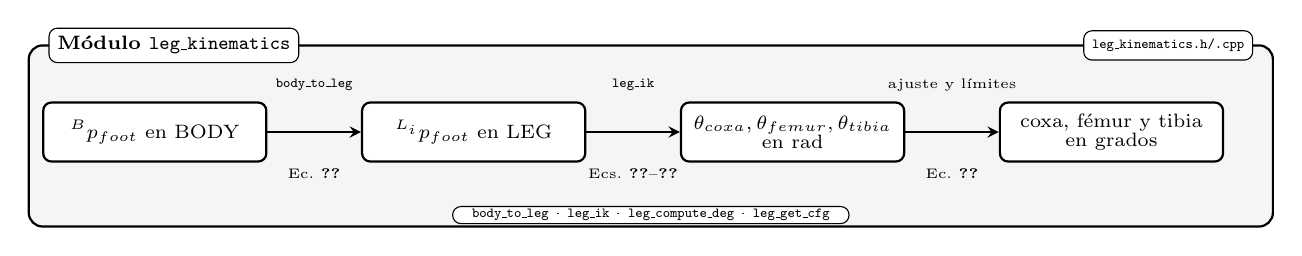
\begin{tikzpicture}[
        >=stealth,
        every node/.style={align=center},
        module/.style={rectangle, rounded corners=5pt, draw=black, thick,
                       fill=gray!8},
        tag/.style={draw=black, rounded corners=3pt, fill=white, inner sep=3pt},
        stage/.style={rectangle, rounded corners=3pt, draw=black, thick,
                      fill=white, text width=2.60cm, minimum height=0.75cm,
                      inner ysep=2pt, font=\scriptsize},
        apibox/.style={rectangle, rounded corners=3pt, draw=black, fill=white,
                       inner xsep=7pt, inner ysep=1pt, font=\tiny},
        note/.style={font=\scriptsize},
        flow/.style={->, thick, draw=black}
    ]

        \draw[module] (-7.90,-0.75) rectangle (7.90,1.55);

        % Cadena de conversión de un objetivo cartesiano en consignas.
        \node[stage] (pb) at (-6.30,0.45) {${}^{B}\bm{p}_{foot}$ en BODY};
        \node[stage] (pl) at (-2.25,0.45) {${}^{L_i}\bm{p}_{foot}$ en LEG};
        \node[stage] (ra) at ( 1.80,0.45) {$\theta_{\text{coxa}},\theta_{\text{femur}},\theta_{\text{tibia}}$\\[-1pt] en rad};
        \node[stage] (dg) at ( 5.85,0.45) {coxa, fémur y tibia\\[-1pt]
                                           en grados};

        \draw[flow] (pb) -- (pl);
        \draw[flow] (pl) -- (ra);
        \draw[flow] (ra) -- (dg);

        % Fila independiente para los nombres de las operaciones.
        \node[font=\tiny] at (-4.275, 1.05) {\texttt{body\_to\_leg}};
        \node[font=\tiny] at (-0.225, 1.05) {\texttt{leg\_ik}};
        \node[font=\tiny] at ( 3.825, 1.05) {ajuste y límites};
        
        % Ecuaciones debajo de la cadena.
        \node[font=\tiny] at (-4.275,-0.08) {Ec.~\ref{eq:Tlb}};
        \node[font=\tiny] at (-0.225,-0.08)
            {Ecs.~\ref{eq:ik_theta}--\ref{eq:theta_tibia}};
        \node[font=\tiny] at ( 3.825,-0.08)
            {Ec.~\ref{eq:calibracion_theta_servo}};

        \node[tag, font=\scriptsize, anchor=west] at (-7.65,1.55)
            {\textbf{Módulo \texttt{leg\_kinematics}}};
        \node[tag, font=\tiny\ttfamily, anchor=east] at (7.65,1.55)
            {leg\_kinematics.h/.cpp};

        \node[apibox, anchor=south] at (0,-0.72)
            {\texttt{body\_to\_leg} · \texttt{leg\_ik} ·
             \texttt{leg\_compute\_deg} · \texttt{leg\_get\_cfg}};

    \end{tikzpicture}}
    \captionsetup{justification=centering,singlelinecheck=false,skip=3pt}
    \caption[Cadena de conversión de \texttt{leg\_kinematics}]
    {Etapas que convierten el objetivo cartesiano en consignas
    angulares.}
    \label{fig:arquitectura_leg_kinematics}
\end{figure}
\vspace{-1.5\baselineskip}

El recorrido comienza con \texttt{body\_to\_leg}, que expresa el objetivo en el
sistema local de la pata mediante la Ec.~\ref{eq:Tlb}. A continuación,
\texttt{leg\_ik} aplica la solución geométrica de la
Subsección~\ref{subsec:theory_ik} y selecciona la rama compatible con el
montaje. Antes de resolverla comprueba la condición
$|L_f-L_t|\leq Hip\leq L_f+L_t$; si el objetivo no es alcanzable, devuelve
\texttt{false}. Finalmente, \texttt{leg\_compute\_deg} convierte la solución a grados y aplica
el ajuste de la Ec.~\ref{eq:calibracion_theta_servo}.

\vspace{-0.5\baselineskip}
\subsection{Estado y comunicación
(\texttt{robot\_controller}/\texttt{serial\_bridge})}
\label{subsec:controller_bridge}
\label{subsec:robot_controller}
\label{subsec:serial_bridge}

Estos módulos forman la interfaz entre la comunicación externa y las tareas de
locomoción y diagnóstico. \texttt{serial\_bridge} traduce los comandos de texto
en operaciones sobre \texttt{robot\_controller}, que centraliza el intercambio
de consignas, odometría y telemetría. De este modo, la comunicación queda
desacoplada (Figura~\ref{fig:controller_bridge}).

\begin{figure}[H]
    \centering
    \makebox[\textwidth][c]{%
    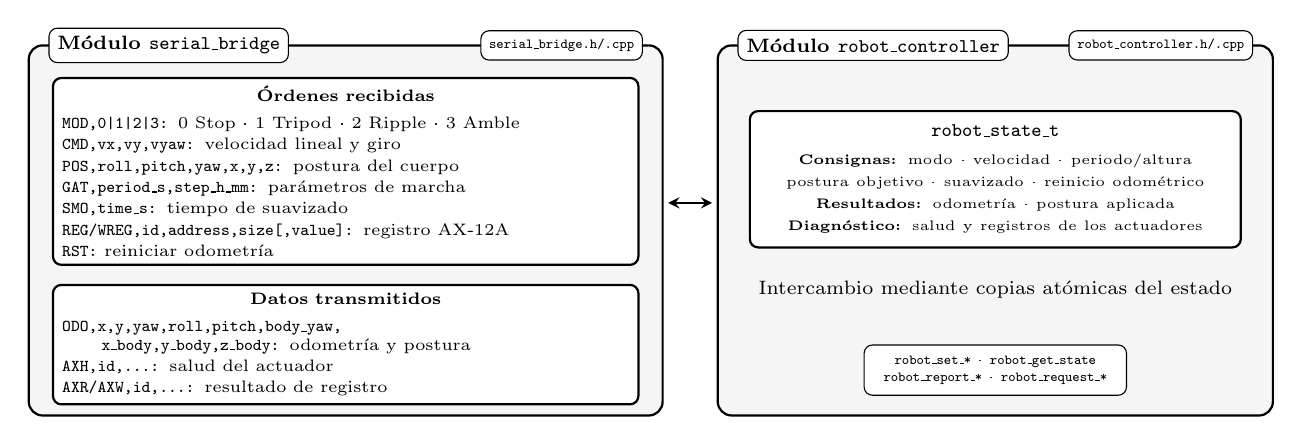
\begin{tikzpicture}[
        >=stealth,
        every node/.style={align=center},
        module/.style={rectangle, rounded corners=5pt, draw=black, thick,
                       fill=gray!8},
        tag/.style={draw=black, rounded corners=3pt, fill=white, inner sep=3pt},
        state/.style={rectangle, rounded corners=3pt, draw=black, thick,
                      fill=white, text width=6.00cm, inner ysep=5pt,
                      font=\scriptsize},
        packet/.style={rectangle, rounded corners=3pt, draw=black, thick,
                       fill=white, text width=7.20cm, align=left,
                       inner ysep=3pt,
                       font=\fontsize{6.5}{7.7}\selectfont},
        apibox/.style={rectangle, rounded corners=3pt, draw=black, fill=white,
                       inner xsep=7pt, inner ysep=4pt, font=\tiny},
        note/.style={font=\scriptsize},
        flow/.style={<->, thick, draw=black}
    ]

        % ---------------- serial_bridge ----------------
        \draw[module] (-7.90,-2.15) rectangle (0.15,2.55);

        \node[packet] (in) at (-3.875,0.95)
            {\makebox[7.20cm][c]{\textbf{Órdenes recibidas}}\\[2pt]
	             \textbf{\texttt{MOD,0|1|2|3:}} 0 Stop · 1 Tripod · 2 Ripple · 3 Amble\\
             \textbf{\texttt{CMD,vx,vy,vyaw:}} velocidad lineal y giro\\
             \textbf{\texttt{POS,roll,pitch,yaw,x,y,z:}} postura del cuerpo\\
             \textbf{\texttt{GAT,period\_s,step\_h\_mm:}} parámetros de marcha\\
             \textbf{\texttt{SMO,time\_s:}} tiempo de suavizado\\
             \textbf{\texttt{REG/WREG,id,address,size[,value]:}} registro AX-12A\\
             \textbf{\texttt{RST:}} reiniciar odometría};
        \node[packet] (out) at (-3.875,-1.25)
            {\makebox[7.20cm][c]{\textbf{Datos transmitidos}}\\[2pt]
             \textbf{\texttt{ODO,x,y,yaw,roll,pitch,body\_yaw,}}\\[-1pt]
             \hspace*{5mm}\textbf{\texttt{x\_body,y\_body,z\_body:}}
             odometría y postura\\
             \textbf{\texttt{AXH,id,...:}} salud del actuador\\
             \textbf{\texttt{AXR/AXW,id,...:}} resultado de registro};

        % ---------------- robot_controller ----------------
        \draw[module] (0.85,-2.15) rectangle (7.90,2.55);
        \node[state] (st) at (4.375,0.85)
            {\texttt{robot\_state\_t}\\[2pt]
             {\tiny \textbf{Consignas:} modo · velocidad · periodo/altura}\\
             {\tiny postura objetivo · suavizado · reinicio odométrico}\\
             {\tiny \textbf{Resultados:} odometría · postura aplicada}\\
             {\tiny \textbf{Diagnóstico:} salud y registros de los actuadores}};

        \node[note] at (4.375,-0.55)
            {Intercambio mediante copias atómicas del estado};
        \node[apibox, anchor=south] at (4.375,-1.90)
            {\texttt{robot\_set\_*} · \texttt{robot\_get\_state}\\
             \texttt{robot\_report\_*} · \texttt{robot\_request\_*}};

        % ---------------- Etiquetas y enlace ----------------
        \node[tag, font=\scriptsize, anchor=west] at (-7.65,2.55)
            {\textbf{Módulo \texttt{serial\_bridge}}};
        \node[tag, font=\tiny\ttfamily, anchor=east] at (-0.10,2.55)
            {serial\_bridge.h/.cpp};
        \node[tag, font=\scriptsize, anchor=west] at (1.10,2.55)
            {\textbf{Módulo \texttt{robot\_controller}}};
        \node[tag, font=\tiny\ttfamily, anchor=east] at (7.65,2.55)
            {robot\_controller.h/.cpp};

        \draw[flow, shorten <=2pt, shorten >=2pt]
            (0.15,0.55) -- (0.85,0.55);

    \end{tikzpicture}}
    \captionsetup{justification=centering,singlelinecheck=false}
    \caption[Intercambio entre el puente serie y el estado compartido]
    {Protocolo propio de comandos de texto y acceso al estado compartido. Las funciones están documentadas con Doxygen~\cite{doxygen}.}
    \label{fig:controller_bridge}
\end{figure}


\texttt{robot\_controller} mantiene el estado compartido del robot, que reúne
las consignas recibidas y los resultados publicados por las tareas internas. Un
mutex protege las operaciones de lectura y escritura. Cada lectura devuelve una
instantánea completa, por lo que las tareas pueden trabajar con datos coherentes
sin mantener el bloqueo.

\texttt{serial\_bridge} se fija al núcleo~0 y ejecuta un bucle sin periodo
estricto. En cada vuelta espera datos de UART durante un máximo de 10~ms,
tiempo durante el cual el núcleo atiende otras tareas. Por ello, sin
tráfico el bucle se repite aproximadamente cada 10~ms, aunque su periodo no es
exacto. Tras procesar una orden, consulta el estado: \texttt{ODO} se envía cada
segundo y \texttt{AXH}, \texttt{AXR} y \texttt{AXW} solo cuando hay datos nuevos.

\newpage
\subsection{Locomoción y diagnóstico
(\texttt{locomotion\_task}/\texttt{diagnostic})}
\label{subsec:locomotion_task}
\label{subsec:diagnostic}

\texttt{locomotion\_task} integra los módulos anteriores en el bucle que genera
las consignas de los 18 actuadores. Esta tarea inicializa y coordina la cadena
cinemática completa, está fijada al núcleo~1 con prioridad~10 y se activa cada
20~ms
(Figura~\ref{fig:arquitectura_locomotion_task}).

\begin{figure}[H]
    \centering
    \makebox[\textwidth][c]{%
    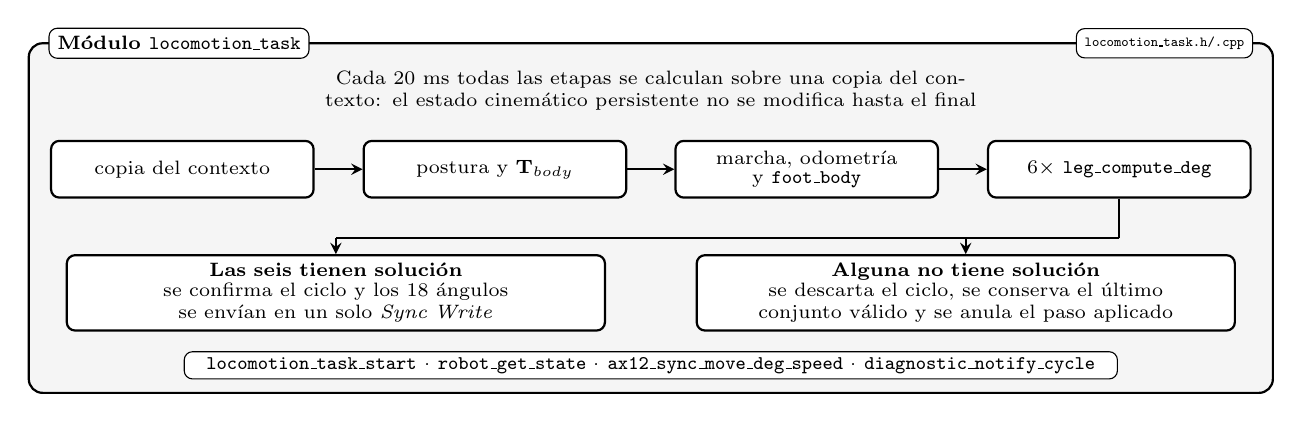
\begin{tikzpicture}[
        >=stealth,
        every node/.style={align=center},
        module/.style={rectangle, rounded corners=5pt, draw=black, thick,
                       fill=gray!8},
        tag/.style={draw=black, rounded corners=3pt, fill=white, inner sep=3pt},
        stage/.style={rectangle, rounded corners=3pt, draw=black, thick,
                      fill=white, text width=3.10cm, minimum height=0.72cm,
                      inner ysep=2pt, font=\scriptsize},
	        result/.style={rectangle, rounded corners=3pt, draw=black, thick,
	                       fill=white, text width=6.60cm, inner ysep=3pt,
	                       font=\scriptsize},
	        apibox/.style={rectangle, rounded corners=3pt, draw=black, fill=white,
	                      inner xsep=8pt, inner ysep=2pt, font=\scriptsize},
	        note/.style={font=\scriptsize},
        flow/.style={->, thick, draw=black}
    ]

	        \draw[module] (-7.90,-2.22) rectangle (7.90,2.22);

	        \node[note, text width=13.0cm] at (0,1.62)
	            {Cada 20~ms todas las etapas se calculan sobre una copia del
	             contexto: el estado cinemático persistente no se modifica hasta
	             el final};

        % Etapas del tick, calculadas sobre la copia
        \node[stage] (c1) at (-5.95,0.62) {copia del contexto};
        \node[stage] (c2) at (-1.98,0.62) {postura y $\mathbf{T}_{body}$};
        \node[stage] (c3) at ( 1.98,0.62) {marcha, odometría\\[-1pt]
                                           y \texttt{foot\_body}};
        \node[stage] (c4) at ( 5.95,0.62) {$6\times$
                                           \texttt{leg\_compute\_deg}};
        \draw[flow] (c1) -- (c2);
        \draw[flow] (c2) -- (c3);
        \draw[flow] (c3) -- (c4);

	        % Confirmación o descarte del ciclo completo
	        \node[result] (ok) at (-4.00,-0.95)
	            {\textbf{Las seis tienen solución}\\[-1pt]
	             se confirma el ciclo y los 18 ángulos se envían
	             en un solo \textit{Sync Write}};
	        \node[result] (ko) at ( 4.00,-0.95)
	            {\textbf{Alguna no tiene solución}\\[-1pt]
	             se descarta el ciclo, se conserva el último conjunto
	             válido y se anula el paso aplicado};

	        \draw[thick] (c4.south) -- (5.95,-0.25);
	        \draw[thick] (5.95,-0.25) -- (-4.00,-0.25);
	        \draw[flow] (-4.00,-0.25) -- (ok.north);
	        \draw[flow] ( 4.00,-0.25) -- (ko.north);

	        \node[tag, font=\scriptsize, anchor=west] at (-7.65,2.22)
	            {\textbf{Módulo \texttt{locomotion\_task}}};
	        \node[tag, font=\tiny\ttfamily, anchor=east] at (7.65,2.22)
	            {locomotion\_task.h/.cpp};

	        \node[apibox, anchor=south] at (0,-2.05)
	            {\texttt{locomotion\_task\_start} · \texttt{robot\_get\_state} ·
	             \texttt{ax12\_sync\_move\_deg\_speed} ·
	             \texttt{diagnostic\_notify\_cycle}};

    \end{tikzpicture}}
	\captionsetup{justification=centering,singlelinecheck=false}
	\caption[Ciclo de locomoción como transacción]
	{Etapas de un ciclo de 20~ms y confirmación conjunta de las seis soluciones
	de cinemática inversa.}
    \label{fig:arquitectura_locomotion_task}
\end{figure}
\vspace{-1\baselineskip}

Antes del bucle, la tarea inicializa el bus DYNAMIXEL a 1~Mbit/s, configura los
actuadores y activa su par. También inicializa el modelo del cuerpo a una altura de 100~mm, las
posiciones neutrales de la Tabla~\ref{tab:neutral_positions} y el patrón trípode;
una orden \texttt{STOP} conserva este patrón con desplazamiento objetivo nulo.

En cada ciclo obtiene una copia atómica de las consignas y otra provisional del
contexto cinemático, sobre la que actualiza la postura, la marcha, la odometría y
las seis IK. Solo si todas son válidas confirma el contexto y envía los 18
ángulos. En caso contrario, conserva el último conjunto válido y anula el paso
aplicado con \texttt{gait\_engine\_halt}, para que una consigna nula permita
reanudar la marcha. Un cambio de
patrón mantiene el objetivo a cero durante dos periodos antes de activar el
nuevo modo. De esta manera se asegura una transición suave. Finalmente, la tarea notifica a \texttt{diagnostic} con
independencia del resultado de la IK, para que se ejecute en la ventana de tiempo restante.

\texttt{diagnostic}, fijada al núcleo~1 con prioridad~9, ejecuta fuera del control periódico las operaciones auxiliares sobre
los servomotores (Figura~\ref{fig:flujo_diagnostic}).

\vspace{-0.35\baselineskip}
\begin{figure}[H]
    \centering
    \makebox[\textwidth][c]{%
    \begin{tikzpicture}[
        >=stealth,
        every node/.style={align=center},
        module/.style={rectangle, rounded corners=5pt, draw=black, thick,
                       fill=gray!8},
        tag/.style={draw=black, rounded corners=3pt, fill=white, inner sep=3pt},
	        box/.style={rectangle, rounded corners=3pt, draw=black, thick,
	                    fill=white, inner ysep=3pt, font=\scriptsize},
	        decision/.style={diamond, aspect=2.4, draw=black, thick, fill=white,
	                         inner sep=1pt, text width=2.60cm, font=\scriptsize},
	        apibox/.style={rectangle, rounded corners=3pt, draw=black, fill=white,
	                      inner xsep=7pt, inner ysep=1pt, font=\tiny},
	        note/.style={font=\scriptsize},
	        flow/.style={->, thick, draw=black}
	    ]

	        \draw[module] (-7.90,-1.95) rectangle (7.90,1.95);

	        \node[note, text width=13.0cm] at (0,1.43)
	            {Se despierta al final de cada ciclo de locomoción y ejecuta una
	             sola transacción};

	        \node[box, text width=2.50cm] (nt) at (-6.10,0.05)
	            {fin del ciclo de locomoción};
	        \node[decision] (q) at (-2.40,0.05)
	            {¿petición nueva?};
	        \node[box, text width=3.20cm] (rg) at (2.20,0.68)
	            {lectura o escritura\\ del registro};
	        \node[box, text width=3.20cm] (hl) at (2.20,-0.55)
	            {salud del siguiente servo};
	        \node[box, text width=2.60cm] (pb) at (6.40,0.05)
	            {publicación en \texttt{robot\_controller}};

        \draw[flow] (nt) -- (q);
        \draw[flow] (q.east) -- node[above, font=\tiny, pos=0.35] {sí} (rg.west);
        \draw[flow] (q.east) -- node[below, font=\tiny, pos=0.35] {no} (hl.west);
        \draw[flow] (rg.east) -- (pb.north);
        \draw[flow] (hl.east) -- (pb.south);

	        \node[note] at (0,-1.20)
	            {una transacción por activación · \textit{timeout} de 8~ms ·
	             ronda de los 18 servos en 360~ms};

	        \node[tag, font=\scriptsize, anchor=west] at (-7.65,1.95)
	            {\textbf{Módulo \texttt{diagnostic}}};
	        \node[tag, font=\tiny\ttfamily, anchor=east] at (7.65,1.95)
	            {diagnostic.h/.cpp};

	        \node[apibox, anchor=south] at (0,-1.78)
	            {\texttt{diagnostic\_start} · \texttt{diagnostic\_notify\_cycle}};

    \end{tikzpicture}}
	\captionsetup{justification=centering,singlelinecheck=false,skip=3pt}
	\caption[Planificación de la tarea de diagnóstico]
	{Selección de una única operación auxiliar después de cada ciclo de
	locomoción.}
    \label{fig:flujo_diagnostic}
\end{figure}
\vspace{-1\baselineskip}

La tarea permanece bloqueada hasta la notificación del final de cada ciclo. En
cada activación atiende primero una petición \texttt{REG}/\texttt{WREG}, si esta no
existe, consulta la tensión, la temperatura, la carga y el error del siguiente
servo de la ronda. Ejecuta como máximo una transacción con un timeout
de 8~ms y publica el resultado en \texttt{robot\_controller}. El mutex interno
de \texttt{ax12} serializa el acceso al bus con la locomoción.

\newpage
\section{Subsistema de alto nivel e integración ROS~2}
\label{sec:integracion_ros2}

Una vez resuelto el control en tiempo real, el subsistema de alto
nivel se plantea como una capa de coordinación, percepción y supervisión. Su cometido
no es ejecutar el control temporal estricto del robot, sino organizar los módulos de
mayor nivel de abstracción y comunicarse de forma desacoplada con el firmware de bajo
nivel. Esta capa se ha desarrollado siguiendo el modelo de
nodos y comunicaciones de ROS~2~\cite{ros2_docs}. Su extensa comunidad y su ecosistema
de paquetes facilitan la integración de sensores, algoritmos de planificación y
control, y herramientas de visualización, además de la modularidad, que permite desarrollar y desplegar cada componente de manera independiente.

\subsection{Interfaz ROS~2 del puente serie}
\label{subsec:ros2_nodes_topics}
\label{subsec:esp32_bridge_ros2}

El primer nodo desarrollado es \texttt{/esp32\_bridge}, incluido en el paquete
\texttt{hexapod\_bridge}. Este nodo constituye la frontera entre dos modelos de
ejecución: hacia ROS~2 ofrece una interfaz basada en mensajes y tópicos, mientras que
hacia el ESP32 mantiene una comunicación UART basada en las órdenes de texto
descritas en la Subsección~\ref{subsec:serial_bridge}. Se trata, en esencia, de un
traductor entre las interfaces de alto nivel y el protocolo del firmware. La interfaz
pública del robot se agrupa bajo el espacio de nombres \texttt{/hexapod}, en el que
se exponen los tópicos recogidos en la Tabla~\ref{tab:ros2_initial_topics}; su
implementación completa está disponible en el repositorio del proyecto
\cite{repositorio_hexapodo}.

\begin{table}[H]
    \centering
    \captionsetup{justification=centering,singlelinecheck=false}
    \scriptsize
    \setlength{\tabcolsep}{3.5pt}
    \renewcommand{\arraystretch}{1.06}
    \rowcolors{2}{black!4}{white}
    \begin{tabularx}{\textwidth}{@{}
        >{\raggedright\arraybackslash}p{3.15cm}
        >{\raggedright\arraybackslash}p{3.25cm}
        >{\centering\arraybackslash}p{1.55cm}
        >{\raggedright\arraybackslash}X @{} }
        \toprule
        \rowcolor{black!14}
        \textbf{Tópico} & \textbf{Mensaje} & \textbf{Sentido} & \textbf{Función} \\
        \midrule
        \path{/hexapod/cmd_vel} &
        \path{geometry_msgs/msg/Twist} &
        \textbf{Entrada} &
        Consigna de velocidad lineal en los ejes $x$ e $y$ y velocidad angular
        alrededor de $z$. \\

        \path{/hexapod/robot_command} &
        \path{std_msgs/msg/String} &
        \textbf{Entrada} &
        Configuración de marcha y postura, reinicio de odometría y acceso a
        registros AX-12A. \\

        \path{/hexapod/odom_model} &
        \path{nav_msgs/msg/Odometry} &
        \textbf{Salida} &
        Odometría teórica calculada a partir del modelo de marcha. \\

        \path{/hexapod/body_pose} &
        \path{geometry_msgs/msg/Pose} &
        \textbf{Salida} &
        Orientación y desplazamiento de cuerpo aplicados por el firmware. \\

        \path{/hexapod/servo_health} &
        \path{std_msgs/msg/String} &
        \textbf{Salida} &
        Tensión, temperatura, carga y alarmas de los 18 actuadores. \\

        \path{/hexapod/servo_register} &
        \path{std_msgs/msg/String} &
        \textbf{Salida} &
        Resultado de una lectura o escritura del mapa de registros AX-12A. \\
        \bottomrule
    \end{tabularx}
    \caption{Interfaz ROS~2 expuesta por el nodo \texttt{/esp32\_bridge}.}
    \label{tab:ros2_initial_topics}
\end{table}
\vspace{-1.0\baselineskip}

\begin{enumerate}[label=\textbf{\arabic*.},leftmargin=*,itemsep=0.4\baselineskip,
                  topsep=0.2\baselineskip,parsep=0.2\baselineskip]
    \item \textbf{Control continuo del movimiento.}
    Las consignas se reciben mediante \path{/hexapod/cmd_vel}. El mensaje
    \texttt{Twist} expresa las velocidades lineales en m/s y la angular en rad/s,
    conforme a las convenciones de ROS~2~\cite{ros2_docs}. El puente convierte las
    primeras a mm/s y calcula las velocidades máximas admisibles a partir del
    recorrido permitido en cada paso y de la duración de la fase de apoyo. Si la
    petición supera los límites calculados, las tres componentes se reducen mediante
    un factor común.

    Por ejemplo, en marcha trípode con un periodo de $2$~s, la fase de apoyo ocupa
    la mitad del ciclo y dura $2\cdot(1/2)=1$~s, de acuerdo con el patrón descrito en
    la Subsección~\ref{subsubsec:gait_patterns}. Con recorridos máximos de $120$~mm
    en $x$, $50$~mm en $y$ y $0{,}35$~rad alrededor de $z$, se obtienen los límites:

    \begingroup
    \setlength{\abovedisplayskip}{0.35\baselineskip}
    \setlength{\belowdisplayskip}{0.35\baselineskip}
    \[
        v_{x,\max}=120~\text{mm/s}, \qquad
        v_{y,\max}=50~\text{mm/s}, \qquad
        \omega_{z,\max}=0{,}35~\text{rad/s}.
    \]
    \endgroup

    Para $(v_x,v_y)=(0{,}12,0{,}05)$~m/s, la demanda normalizada vale
    $120/120+50/50=2$ y el factor $1/2$ produce $(v_x,v_y)=(60,25)$~mm/s, conservando la dirección.

    \item \textbf{Configuración y diagnóstico.}
    Las operaciones discretas se reciben mediante
    \path{/hexapod/robot_command}. Este tópico transporta cambios de modo
    (\texttt{MOD}), periodo y altura de paso (\texttt{GAT}), postura
    (\texttt{POS}), suavizado (\texttt{SMO}), reinicio de odometría y accesos a los
    registros de los actuadores (\texttt{REG}/\texttt{WREG}). Las órdenes
    \texttt{CMD} se descartan expresamente en este canal, de modo que el movimiento
    solo pueda introducirse mediante la interfaz estándar \texttt{Twist}. Los cambios
    de marcha se conservan localmente porque condicionan los límites aplicados a las
    consignas posteriores.

    \item \textbf{Publicación de telemetría.}
    En el sentido ESP32--ROS~2, el puente lee continuamente la UART y clasifica cada
    línea por su prefijo. Una trama \texttt{ODO} origina dos publicaciones:
    \path{/hexapod/odom_model} contiene la traslación planar y la orientación
    estimadas, mientras que \path{/hexapod/body_pose} representa la postura aplicada
    al cuerpo. Las posiciones se convierten de milímetros a metros y los ángulos se
    expresan mediante cuaterniones. Las tramas \texttt{AXH} se publican como estado de
    los actuadores, y las respuestas \texttt{AXR}/\texttt{AXW}, como resultados del
    acceso a sus registros.
\end{enumerate}

La interfaz no fija qué nodos deben utilizarla: cualquier publicador que respete los
tipos establecidos puede enviar consignas y cualquier suscriptor puede consumir la
telemetría. Como ejemplo, la Figura~\ref{fig:ros2_teleop_graph} muestra
\texttt{/teleop\_twist\_keyboard}~\cite{ros2_teleop_twist_keyboard} publicando
mensajes \texttt{geometry\_msgs/msg/Twist} en \path{/hexapod/cmd_vel}.


\begin{figure}[H]
    \centering
    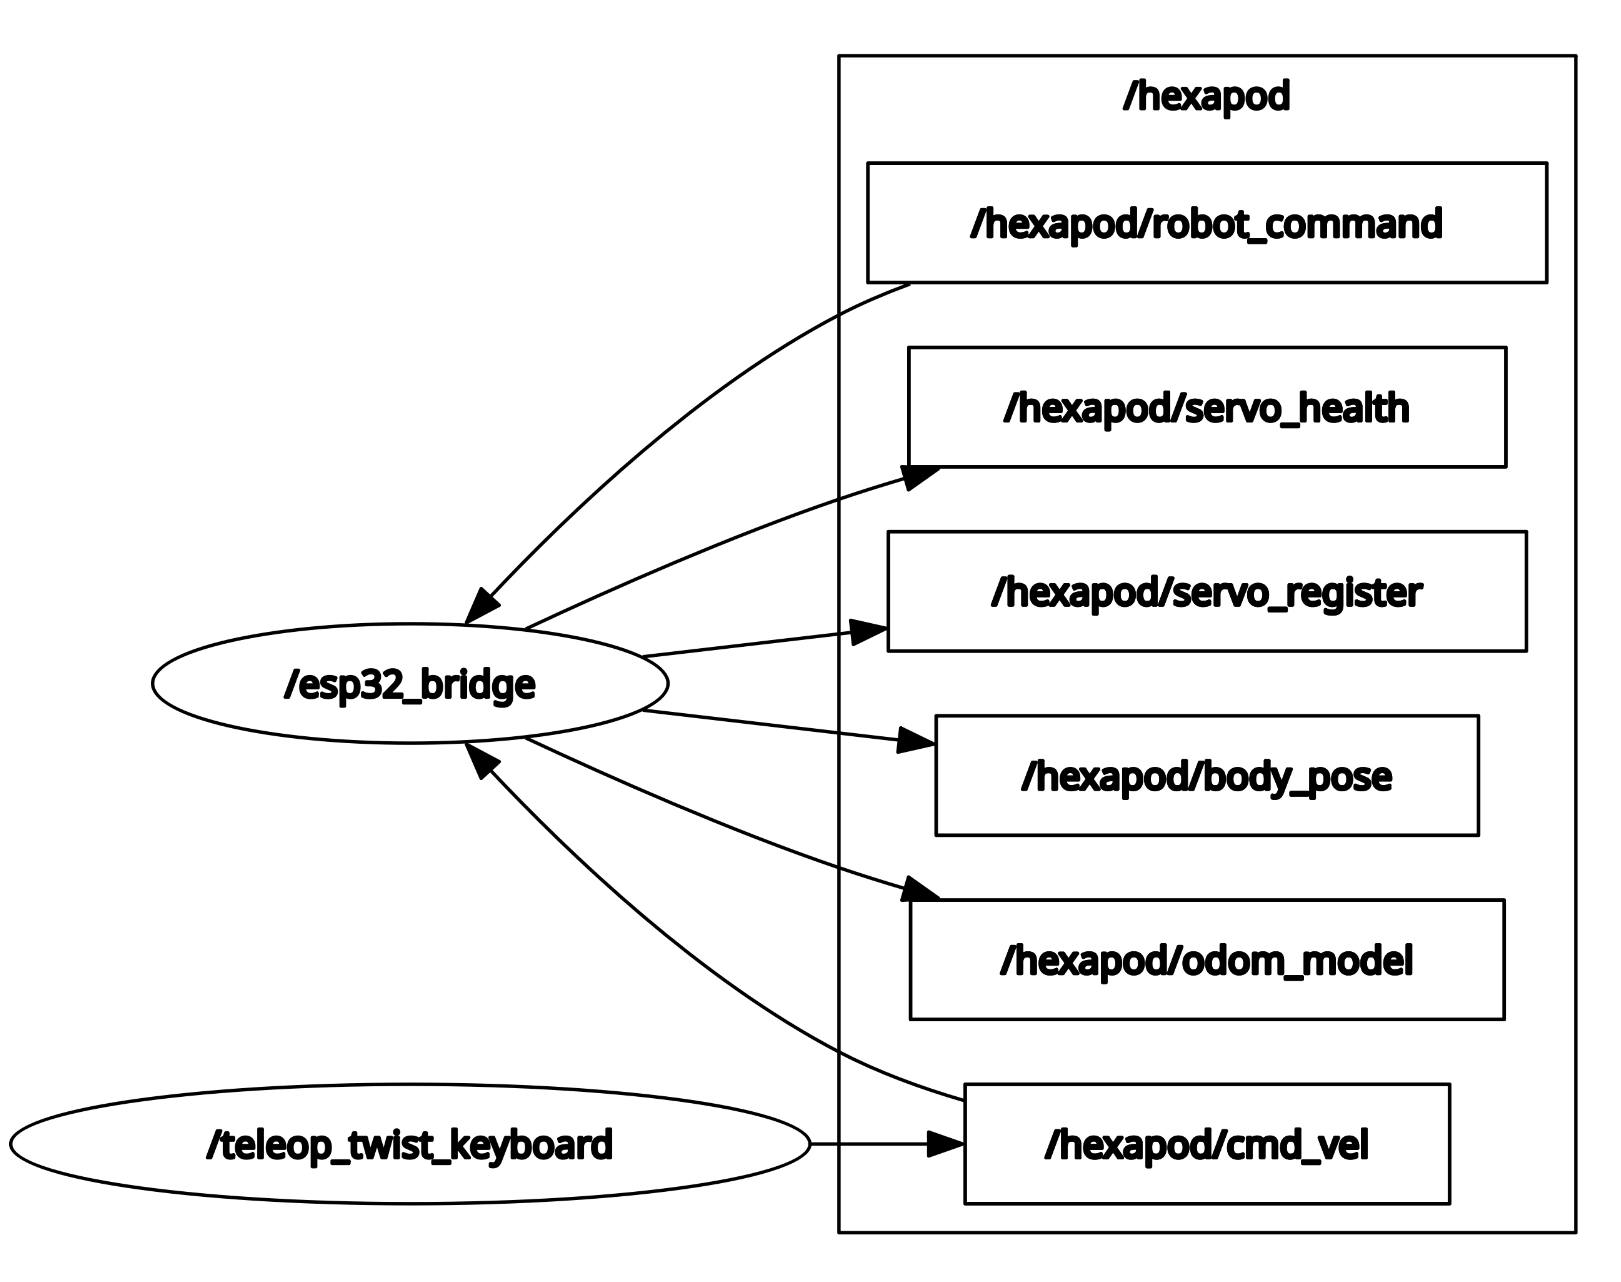
\includegraphics[width=0.75\textwidth]{capitulos/cap3/figuras/ros2_rqt_teleop.png}
    \captionsetup{justification=centering,singlelinecheck=false}
    \caption[Teleoperación mediante una interfaz ROS~2 estándar]
    {Conexión de \texttt{/teleop\_twist\_keyboard} con \texttt{/esp32\_bridge}
    mediante \texttt{/hexapod/cmd\_vel}, visualizada con \texttt{rqt\_graph}.}
    {\centering\footnotesize Fuente: Elaboración propia.\par}
    \label{fig:ros2_teleop_graph}
\end{figure}
\vspace{-1.0\baselineskip}

Otra integración habitual en este tipo de soluciones consiste en conectar
periféricos externos mediante paquetes de adaptación. En el caso de un mando de
videojuegos, el paquete \texttt{joy}~\cite{ros2_joy} publica su estado mediante mensajes
\path{sensor_msgs/msg/Joy}, lo que ofrece otra posible vía de
integración. Sin embargo, la necesidad de disponer de una interfaz que se adaptase al
conjunto de tópicos y que, a su vez, sirviera como herramienta de supervisión, llevó a desarrollar un panel web específico, que se describe en la
Subsección~\ref{subsec:web_panel_ros2}.

\clearpage
\subsection{Panel web como cliente de la interfaz del hexápodo}
\label{subsec:web_panel_ros2}

El panel web se desarrolló como un cliente de la interfaz proporcionada por \texttt{/esp32\_bridge}. Su nodo \texttt{/web\_panel} convierte las acciones del
navegador en publicaciones ROS~2 y presenta la telemetría recibida mediante sus
suscripciones. De este modo, reúne el control, la configuración y la supervisión sin
modificar la interfaz del puente. La relación entre ambos nodos se muestra en la
Figura~\ref{fig:ros2_rqt_graph}, y sus vistas se recogen a mayor tamaño en el
\hyperref[anexo:capturas_panel_web]{Anexo~E}.

\begin{figure}[H]
    \centering
    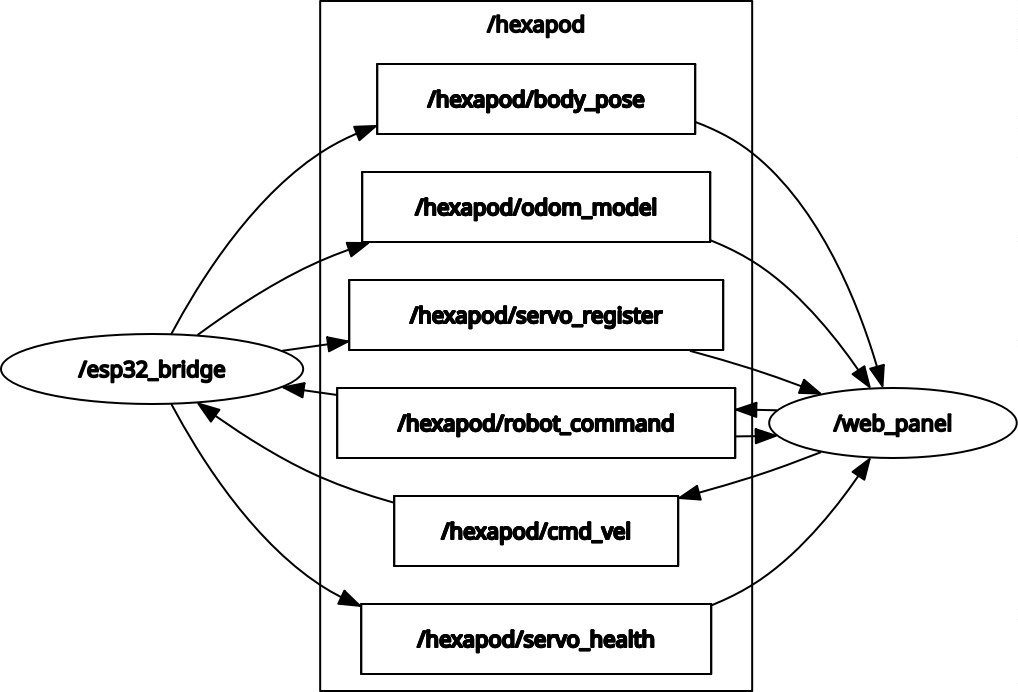
\includegraphics[width=0.75\textwidth]
        {capitulos/cap3/figuras/ros2_rqt_graph.png}
    \captionsetup{justification=centering,singlelinecheck=false}
    \caption[Panel web como cliente de la interfaz ROS~2]
    {Conexión del panel web con la interfaz de \texttt{/esp32\_bridge}.}
    {\centering\footnotesize Fuente: Elaboración propia.\par}
    \label{fig:ros2_rqt_graph}
\end{figure}
\vspace{-1.4\baselineskip}

\begin{enumerate}[label=\textbf{\arabic*.},leftmargin=*,
                  itemsep=0.25\baselineskip,topsep=0.15\baselineskip]
    \item \textbf{Control del movimiento y configuración de la marcha.}
    El bloque de teleoperación de la Figura~\ref{fig:anexo_web_panel_general} ofrece
    un área de control bidimensional para las velocidades $v_x$ y $v_y$, un deslizador independiente para el giro y campos numéricos con los
    que introducir consignas precisas. Desde ella se seleccionan también los modos
    \textit{tripod}, \textit{ripple} y \textit{amble}, el periodo y la altura de paso.
    Mientras existe un modo de marcha activo, \texttt{/web\_panel} publica la velocidad
    en \path{/hexapod/cmd_vel} a 10~Hz. Esa renovación periódica actúa además como
    señal de actividad: si el puente no recibe una consigna nueva antes de un segundo,
    la considera caducada y ordena velocidad nula, de modo que el robot se detiene si
    el navegador deja de responder. Los cambios discretos de modo y de parámetros, en
    cambio, se envían una sola vez mediante \path{/hexapod/robot_command}.

    \item \textbf{Postura y supervisión del movimiento.}
    Esa misma vista permite ajustar los tres ángulos de orientación y los tres
    desplazamientos del cuerpo, junto con el tiempo de suavizado de postura. Para cada componente se presentan conjuntamente el objetivo
    solicitado y el valor aplicado que el firmware publica en
    \path{/hexapod/body_pose}.

    \item \textbf{Diagnóstico de los actuadores.}
    El panel de la Figura~\ref{fig:anexo_web_panel_servos} distribuye los 18 actuadores según su
    posición en el robot y presenta, para cada uno, su identificador, articulación,
    temperatura, carga y tensión. Al seleccionar uno se abre la tabla de registros
    AX-12A de la Figura~\ref{fig:anexo_web_panel_registers}, desde la que pueden
    consultarse todos ellos y escribirse únicamente los que la aplicación habilita. Las
    solicitudes utilizan \path{/hexapod/robot_command} y las respuestas,
    \path{/hexapod/servo_register}.
\end{enumerate}



\clearpage
\subsection{Percepción y navegación reactiva}
\label{subsec:lidar_ros2}



Dotar a la plataforma de percepción del entorno es el paso previo a cualquier interacción. Este trabajo no aborda un sistema de navegación completo, pero demuestra
la integración de un sensor con un algoritmo como base
para una futura planificación.

\begin{wrapfigure}[14]{r}{0.45\textwidth}
  \vspace{-0.3\baselineskip}
  \centering
  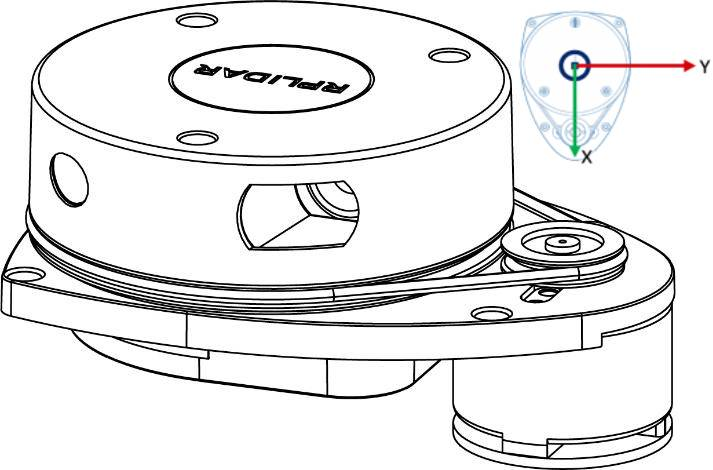
\includegraphics[width=1\linewidth]{capitulos/cap3/figuras/rplidar_a1m8.jpg}
  \captionsetup{justification=centering}
  \caption{LiDAR RPLIDAR~A1M8 y su sistema de referencia angular.}
  \footnotesize Fuente: SLAMTEC~\cite{rplidar_a1m8_datasheet} y
  \texttt{sllidar\_ros2}~\cite{sllidar_ros2}.
  \label{fig:rplidar_a1m8}
\end{wrapfigure}

El sensor empleado es el LiDAR RPLIDAR~A1M8 \cite{rplidar_a1m8_datasheet}, introducido
en la Sección~\ref{sec:arquitectura_general} y conectado por USB a la Raspberry~Pi~4.
Este LiDAR proyecta un haz láser y, mediante un sensor de imagen
desplazado respecto al emisor, registra la posición del punto reflejado, de cuya
geometría se deduce la distancia. La integración en ROS~2 corre a cargo de \texttt{sllidar\_ros2}
\cite{sllidar_ros2}, el controlador que mantiene el propio fabricante. Su nodo
\texttt{/sllidar\_node} admite como parámetros el puerto serie, la velocidad de
transmisión, el identificador del sistema de referencia y el modo de barrido.

El nodo publica una única salida, el tópico \path{/scan}, con mensajes
\path{sensor_msgs/msg/LaserScan}, el tipo estándar de ROS~2 \cite{ros2_docs}. El
ángulo cero de la medida no lo decide el software, sino una referencia física
solidaria a la carcasa del sensor (Figura~\ref{fig:rplidar_a1m8}), que debe quedar
alineada con el frente del robot al montarlo. El controlador se limita a reordenar las
medidas para seguir el convenio de ROS~2, con el ángulo creciente en sentido
antihorario entre $-\pi$ y $\pi$~rad. De ahí que la medida $i$-ésima corresponda a
$\theta_i=\theta_{\min}+i\,\Delta\theta$ (el índice cero del vector \path{ranges}
apunta hacia atrás y el sector frontal cae en la mitad central del vector).

El sensor se ha atornillado de modo que su eje~Y (el de ángulo cero) quede alineado
con el eje~X del sistema del cuerpo $\{B\}$ definido en la
Subsección~\ref{subsec:frames_notacion} (Figura~\ref{fig:coordenadascoxas}), es
decir, con el frente del robot. La Figura~\ref{fig:rviz2_scan} muestra un barrido obtenido con esta configuración.


\begin{figure}[H]
    \vspace{-2.3pt}
    \centering
    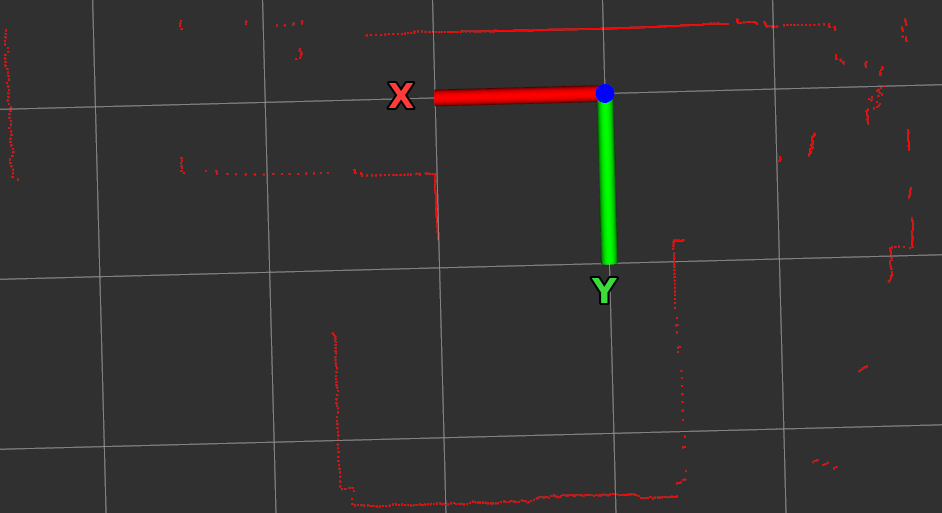
\includegraphics[width=0.8\textwidth]{capitulos/cap3/figuras/rviz2_scan_lidar.png}
    \captionsetup{justification=centering,singlelinecheck=false}
    \caption[Barrido del RPLIDAR~A1M8 visualizado en RViz~2]
    {Nube de puntos publicada en \texttt{/scan} y visualizada en RViz~2, con los
    ejes del sistema del cuerpo etiquetados.}
    {\centering\footnotesize Fuente: Elaboración propia.\par}
    \label{fig:rviz2_scan}
\end{figure}

\paragraph{Filtrado del barrido}

Antes de llegar al evitador, cada barrido atraviesa el nodo
\texttt{/scan\_to\_scan\_filter\_chain} del paquete \texttt{laser\_filters}
\cite{laser_filters}, que encadena dos filtros y publica el resultado en
\path{/scan_filtered}. Cuando el RPLIDAR~A1M8 no recibe eco, el controlador
publica una distancia infinita. En interiores, esa ausencia rara vez corresponde
a espacio libre, sino a superficies oscuras o transparentes, a incidencias
rasantes o a objetos más próximos que el alcance mínimo del sensor, de 0,15~m
\cite{rplidar_a1m8_datasheet}. Por ello, el primer filtro
(\texttt{InterpolationFilter}) sustituye cada tramo sin eco por la media de las
medidas válidas que lo delimitan, de modo que un cristal o un objeto oscuro
situado entre dos zonas con eco se percibe como un obstáculo. El segundo
(\texttt{LaserScanSpeckleFilter}) descarta las medidas a menos de 1~m que no
forman parte de un grupo de tres medidas consecutivas con diferencias inferiores
a 0,1~m, lo que suprime los retornos espurios aislados sin eliminar objetos
delgados reales. El orden es deliberado: aplicados a la inversa, los ecos
aislados de un objeto oscuro se descartarían antes de servir de referencia a la
interpolación y el objeto desaparecería del barrido.

\paragraph{Evitador reactivo}

Sobre \path{/scan_filtered} se ha implementado un evitador de obstáculos
reactivo, inspirado en los controladores de tres sectores habituales en robótica
móvil. No construye mapas ni planifica trayectorias: en cada barrido toma una
única decisión. Su nodo, \texttt{/reactive\_node}, pertenece al paquete
\texttt{obstacle\_avoider}.

El robot se modela como un círculo de 0,35~m de radio centrado en el LiDAR, que
contiene los pies durante la marcha, pues estos no se alejan más de 0,294~m del
centro. De cada barrido se extraen cuatro distancias: la libre a lo largo del
pasillo frontal, franja de 0,7~m de ancho que el robot barrería al avanzar, y la
de la medida más cercana en los sectores laterales izquierdo y derecho (de
$35^\circ$ a $120^\circ$) y en el entorno completo. El pasillo sustituye al
sector frontal cónico habitual, que se estrecha junto al robot y deja fuera los
obstáculos situados delante de las patas delanteras. Un sector sin medidas
válidas se considera ocupado. Con estas distancias, el nodo aplica las reglas
siguientes, que resume la Figura~\ref{fig:evitador_sectores}:

\begin{enumerate}[label=\textbf{\arabic*.},leftmargin=*,
                  itemsep=0.25\baselineskip,topsep=0.15\baselineskip]
    \item \textbf{Avance.} Si el pasillo frontal dispone de al menos 0,5~m libres,
    el robot avanza a 0,08~m/s y corrige el rumbo para separarse de las paredes
    laterales situadas a menos de 0,8~m, con una velocidad angular proporcional a
    la diferencia entre ambos lados y limitada a 0,25~rad/s.

    \item \textbf{Giro.} Si el pasillo está ocupado pero el círculo del robot está
    libre, este gira sobre sí mismo a 0,25~rad/s hacia el lateral más despejado
    hasta que el pasillo vuelve a quedar libre. El sentido se elige al iniciar el
    giro y se mantiene hasta reanudar el avance, para lo que se exigen 0,6~m en
    lugar de 0,5~m. Esta histéresis evita que pequeñas variaciones entre barridos
    consecutivos hagan alternar al robot entre avanzar y girar, o entre ambos
    sentidos de giro.

    \item \textbf{Parada.} Si alguna medida cae dentro del círculo del robot, se
    ordena velocidad nula, ya que un giro sobre sí mismo podría llevar una pata
    contra el obstáculo. Esta condición supone que el LiDAR se encuentra centrado
    en el cuerpo.
\end{enumerate}

\begin{figure}[H]
    \centering
    \makebox[\textwidth][c]{%
    \begin{tikzpicture}[
        >=stealth,
        every node/.style={align=center},
        module/.style={rectangle, rounded corners=5pt, draw=black, thick,
                       fill=gray!8},
        tag/.style={draw=black, rounded corners=3pt, fill=white, inner sep=3pt},
        box/.style={rectangle, rounded corners=3pt, draw=black, thick,
                    fill=white, inner ysep=3pt, font=\scriptsize},
        dec/.style={diamond, draw=black, thick, fill=white, inner sep=1pt,
                    font=\scriptsize},
        apibox/.style={rectangle, rounded corners=3pt, draw=black, fill=white,
                       inner xsep=7pt, inner ysep=4pt, font=\tiny},
        flow/.style={->, thick, draw=black}
    ]

        \draw[module] (-7.90,-4.10) rectangle (7.90,3.55);

        % ---------------- Sectores (escala 1 m = 5 cm, X_B hacia arriba) ----------------
        \begin{scope}[shift={(-4.10,-0.35)}, scale=5]
            % Laterales: de 35 a 120 grados a cada lado
            \fill[gray!22, draw=black] (0,0) -- (125:0.70)
                arc[start angle=125, end angle=210, radius=0.70] -- cycle;
            \fill[gray!22, draw=black] (0,0) -- (-30:0.70)
                arc[start angle=-30, end angle=55, radius=0.70] -- cycle;
            % Pasillo frontal: ancho del robot (0,7 m) hasta el umbral de avance
            \fill[gray!50, draw=black] (-0.35,0) rectangle (0.35,0.50);
            % Círculo del robot: debe estar libre para girar
            \draw[thick, dashed] (0,0) circle[radius=0.35];
            % Círculo que contiene los pies durante la marcha y LiDAR en el centro
            \draw[thick, fill=white] (0,0) circle[radius=0.294];
            \draw[->, thick] (0,0) -- (0,0.15) node[right, font=\tiny, inner sep=1pt] {$X_B$};
            \draw[->, thick] (0,0) -- (-0.15,0) node[above left, font=\tiny, inner sep=1pt] {$Y_B$};
            \fill (0,0) circle[radius=0.012];

            \node[font=\tiny] at (90:0.61)
                {pasillo frontal ($0{,}7$~m)\\avance desde $0{,}5$~m};
            \node[font=\tiny] at (167.5:0.56) {lateral\\izquierdo};
            \node[font=\tiny] at (12.5:0.56) {lateral\\derecho};
            \node[font=\tiny, fill=gray!8, inner sep=1pt] at (0,-0.47)
                {círculo del robot: $0{,}35$~m};
        \end{scope}

        % ---------------- Reglas de decisión ----------------
        \node[dec, aspect=2.6, text width=1.70cm] (d1) at (2.35,2.25)
            {¿pasillo\\$\geq 0{,}5$~m?};
        \node[box, text width=2.60cm] (adv) at (6.25,2.25)
            {\textbf{Avance} a $0{,}08$~m/s\\[-1pt] con corrección lateral};

        \node[dec, aspect=2.6, text width=1.70cm] (d2) at (2.35,0.25)
            {¿círculo\\libre?};
        \node[box, text width=2.60cm] (stop) at (6.25,0.25)
            {\textbf{Parada}\\[-1pt] velocidad nula};

        \node[box, text width=5.00cm] (turn) at (3.55,-1.75)
            {\textbf{Giro} a $0{,}25$~rad/s hacia el lateral más\\[-1pt]
             despejado hasta liberar $0{,}6$~m de pasillo};

        \draw[flow] (d1) -- node[above, font=\tiny] {sí} (adv);
        \draw[flow] (d1) -- node[right, font=\tiny] {no} (d2);
        \draw[flow] (d2) -- node[above, font=\tiny] {no} (stop);
        \draw[flow] (d2.south) -- node[right, font=\tiny] {sí} (d2.south |- turn.north);

        % ---------------- Etiquetas del módulo ----------------
        \node[tag, font=\scriptsize, anchor=west] at (-7.65,3.55)
            {\textbf{Nodo \texttt{/reactive\_node}}};
        \node[tag, font=\tiny\ttfamily, anchor=east] at (7.65,3.55)
            {reactive\_node.py};

        \node[apibox, anchor=south] at (0,-3.95)
            {entrada \texttt{/scan\_filtered} · salida \texttt{/obstacle\_avoider/cmd\_vel} ·
             una decisión por barrido};

    \end{tikzpicture}}
    \captionsetup{justification=centering,singlelinecheck=false}
    \caption[Zonas y reglas del evitador reactivo]
    {Pasillo frontal, sectores laterales y círculo del robot en el sistema del
    cuerpo $\{B\}$, y reglas de decisión aplicadas en cada barrido.}
    \label{fig:evitador_sectores}
\end{figure}
\vspace{-1\baselineskip}

